\chapter{基于图文对比对抗训练的神经机器翻译}
% 本章要强调 隐式方法在理论上对视觉信息的利用率最大,能够最大程度提升翻译,但实际研究中却很难实现
% 已有工作
前两章聚焦于图片信息增强式的神经翻译模型,通过在模型训练阶段引入视觉信息可以增强模型的表示能力,从而提升纯文本翻译模型的翻译质量。
% 存在的问题
然而这类方法主要针对在模型推理阶段不需要输入图片的情况,当句子中存在病句问题时,需要在翻译的过程中使用图片信息辅助翻译模型解决文本信息存在的问题。
%然而这种做法规避了图片信息在生成翻译过程中的辅助作用,使得视觉信息的作用没有得到充分的发挥。
% 本章所针对的问题
为此本章主要探索图片信息辅助式的神经机器翻译方法,尝试将图片信息融入句子级别的语义信息中。在针对已有方法的讨论中可知,此类方法主要采用隐式跨模态信息融合方法,需要解决神经机器翻译模型对视觉信息不敏感的问题。
% 具体做法
因此,本章提出了一种图文对比对抗训练方法,尝试提升视觉信息在语义表示学习过程中的参与度。在模型输入为文本加图片的情况下,通过与图文对抗样本进行对比,使模型重视图片输入信息与文本描述之间的差异,并将图片信息融合到文本的表示中。
% 结果
在英德翻译、英日翻译和英印翻译三个翻译任务上的实验表明,本章所提方法能够有效提升翻译准确率的同时,增强了模型对视觉信息的敏感度。

\section{引言}
% 大背景(跳过)
% 相关方法的做法,这里应该强调的是guide,还有就是句子级的语义融合
% 图片中往往包含了更完整更丰富的语义信息,因此为了得到更准确的翻译,在翻译过程中加入图片信息成为了一种可行的方案。为了将图片信息融合到翻译中,广大研究者付出了很多的努力。早期的相关研究尝试在句子的编码过程中输入图片使编码结果更接近真实的语义,例如将图片特征作为基于RNN的翻译模型的初始化向量【】,亦或是将图片作为一个单词输入到模型中。也有一些方法以图片特征作为语义的中枢点,尝试为来自不同语言的文字或不同模态的语义信息创造一个统一的语义空间【】。同时,也有方法尝试在解码阶段输入图片,从而引入更多可参考的信息使解码的结果更准确。例如文献【】采用了注意力机制,在基于RNN或是基于Transformer的方法中均有着相似的应用。也有方法尝试
图片中往往包含着相比于文本描述更丰富的语义信息,因此为了得到更准确的翻译,在翻译过程中加入图片信息成为了一种可行的方案。为了将图片信息融合到翻译中,广大研究者付出了很多的努力。早期的相关研究尝试在句子的编码过程中输入图片使编码结果更接近真实的语义,例如将图片特征作为基于循环神经网络的翻译模型的初始化向量\pcite{elliott2015multilanguage,calixto2017incorporating},亦或是作为一个单词输入到模型中。也有一些方法以图片特征作为语义的中枢点,尝试为来自不同语言的文字或不同模态的语义信息创造一个统一的语义空间\pcite{kiros2014unifying,nakayama2017zero}。同时,也有方法尝试在解码阶段输入图片,从而引入更多可参考的信息使解码的结果更准确\pcite{calixto2017doubly,libovicky2018input}。这些方法普遍以句子为语义单位融合图片信息,这样做能够更充分地利用图片所包含的语义,也能最大化的辅助翻译过程。

%存在问题
然而,无论是通过简单地将图片输入翻译模型或是对模型结构进行复杂的设计,图片信息都很难为翻译带来理想的效果。一方面,输入图片信息不能够保证为翻译带来性能的提升;另一方面,当为待翻译句子提供与其内容不一致的图片时,对实际的翻译结果影响很小。这些问题说明一般的神经机器翻译模型对输入图片所提供的视觉信息并不敏感。

%本文做法
\begin{figure}[!htbp]
    \centering
    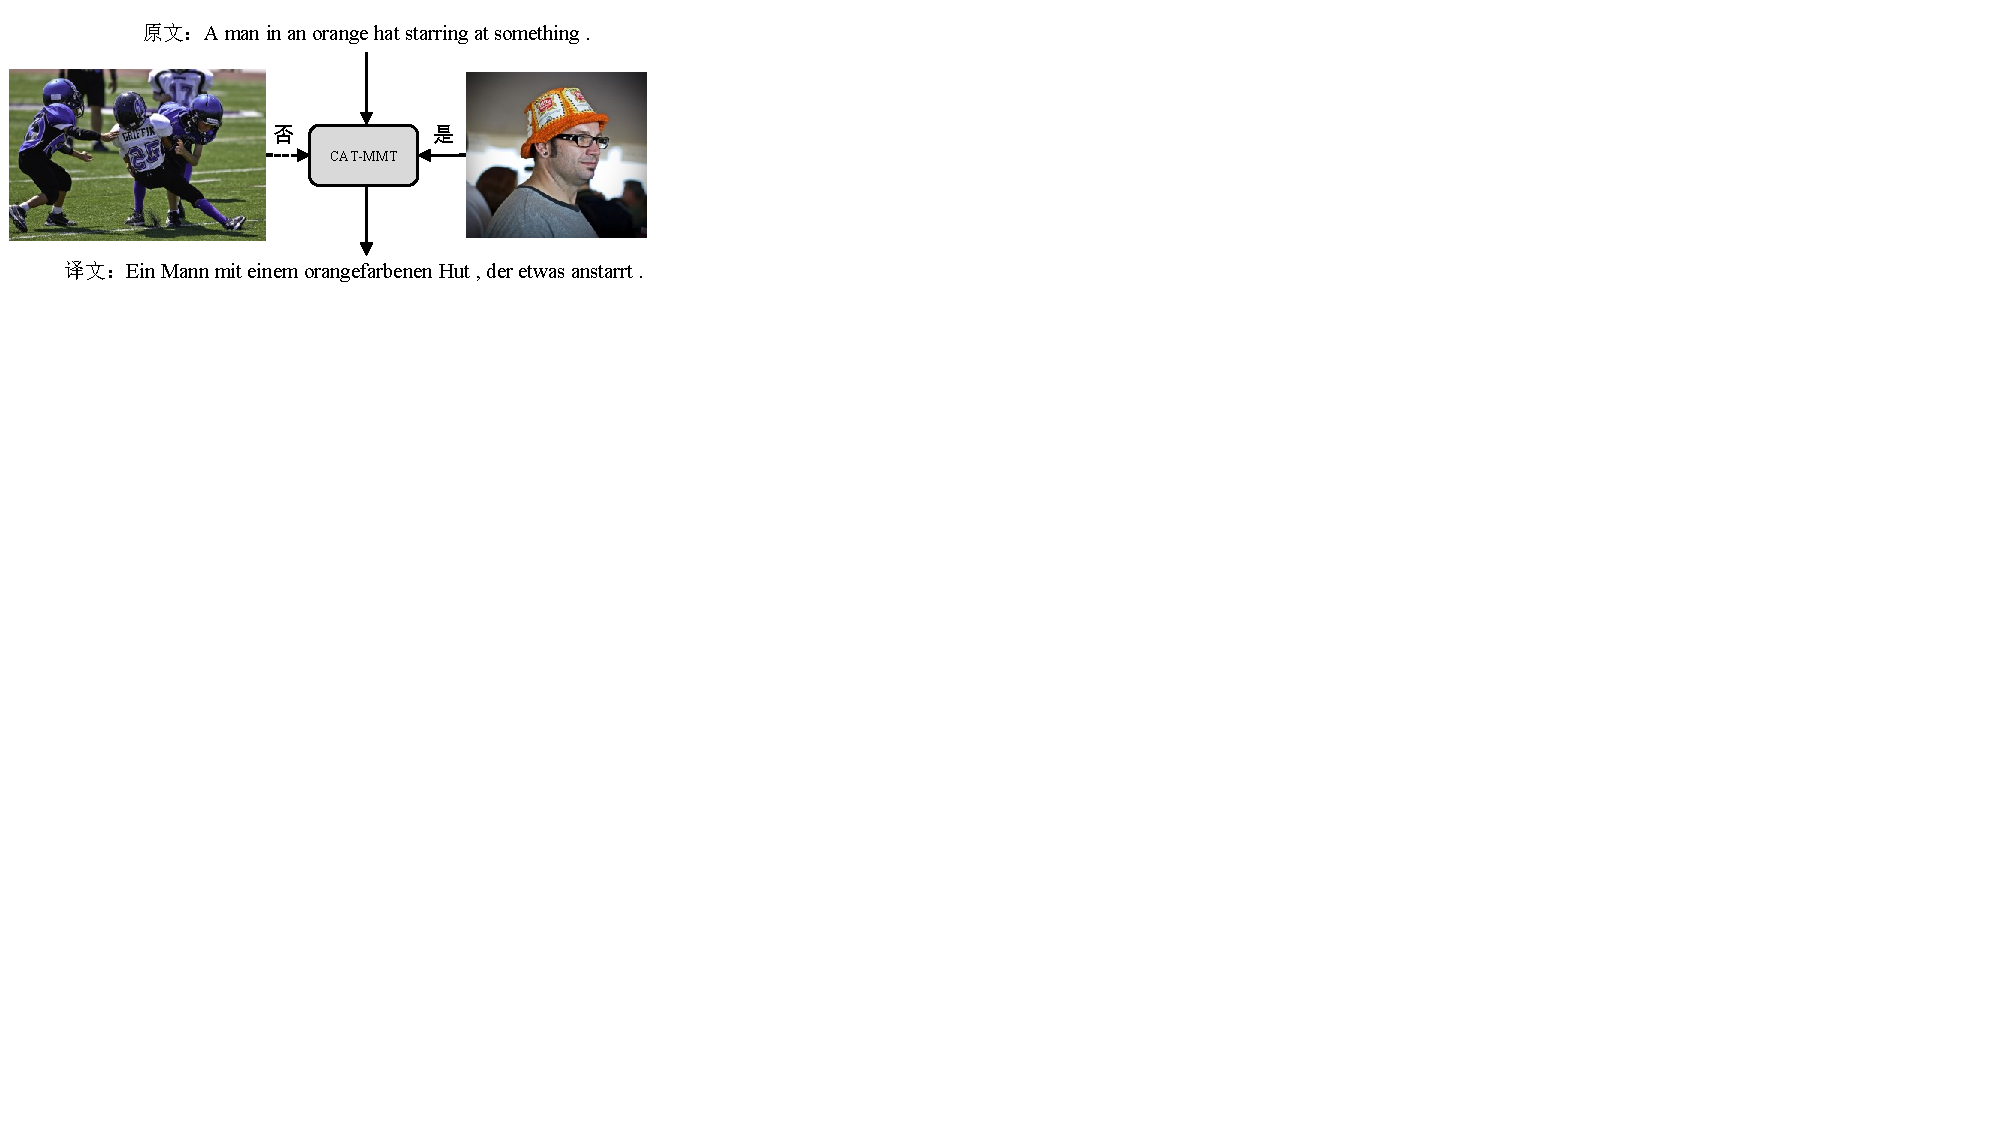
\includegraphics{Img/fig_5_example.pdf}
    \bicaption{引入对抗样本的神经机器翻译模型}{NMT model with adversarial samples}
    \label{fig:5_example}
\end{figure}
已有的相关工作表明在神经机器翻译任务中实现句子级的跨模态语义信息融合是很困难的。只有少部分的待翻译句子需要额外的输入图片作为信息的补充。大部分的翻译数据已经具备良好的双语对齐关系,这使得融合图片信息的端到端模型在面对更容易学习的并且是文本主导的翻译任务时,并不会过多地关注跨模态的信息对齐与融合。因此,针对神经机器翻译中的句子级跨模态语义融合方法,在讨论图片信息是否以及在哪些方面能够为翻译带来质量提升之前,应该更多地关注如何使模型具备从两个模态共同获得信息的能力。为此,本章提出了一种对比对抗训练(contrastive adversarial training, CAT)方法用于解决这个问题。首先,本章的模型输入与一般融合图片信息的翻译模型相似,为一个源语言句子和一张对应的图片。其中该图片中的视觉目标被提取出来,并一同输入到模型中。然后采用对比学习的方法拉近输入与译文在统一语义表示空间的距离。其中,译文作为锚点(anchor),将源语言句子与对应图片组合而成的图文输入作为正样本。为了使模型关注到图片所携带的视觉信息,本章将源语言句子与随机图片组合而成的图文输入作为负样本。如图\ref{fig:5_example}所示,应用该策略可以强迫翻译模型关注输入的源语言文本与输入图片的语义关系,从而实现句子级别的跨模态信息融合。

%具体贡献
本章主要贡献如下:

% 主要翻译性能上的贡献
(1)本章提出了一种基于图文对比对抗训练的神经机器翻译方法,又称CAT-NMT。在配合双向翻译训练后,对比对抗训练能够有效地为图片信息辅助式的神经机器翻译方法带来翻译准确率的提升。该方法在三个不同的翻译数据上得到了有效的提升。

% 主要动机上的贡献
(2)本章所提方法旨在将视觉信息融合到本文的表示中,
%试图通过图片信息加强翻译模型在编码过程中对源语言文本的表示能力,
试图利用图片信息辅助模型编码器完善对源语言文本的表示,
从而提升最终翻译的质量。在对抗实验的分析中可以观察到,CAT-NMT的翻译质量提升来源于成功地将图片信息融合到了文本表示中。因此,CAT方法达到了使神经机器翻译模型对视觉信息敏感的目的。

% 分析结果的贡献
(3)在对模型结果的分析中发现,为翻译输入随机图片或不输入图片时,带有歧义词较多的测试集受到的影响最大。该结果可以表明当神经机器翻译模型对视觉信息敏感时,对文本中存在歧义词问题的句子具有更好的翻译效果。
\section{相关工作}
%本章工作主要针对将加入对抗样本的对比学习方法应用到融合图片信息的神经机器翻译中,因此相关工作可以分为以下三个部分:
本章工作主要采用在对比学习方法中加入对抗样本的方式,迫使模型将图片信息融合到文本表示中。因此,相关工作可以分为以下三个部分:

%传统方法:都有哪些方法,这些方法出现的问题,
{\sffamily (1)图片信息辅助式神经机器翻译}
%这里指出简单的方法,和复杂的方法
在融合图片信息的神经机器翻译方法中,将图片作为翻译模型输入的一部分,并将其用于辅助源语言文本的编码,或在目标语言生成过程中提供外源参考信息的图片辅助式神经机器翻译是目前最常见的一类。图片可以以多种方式与神经翻译任务相结合,而为了更有效地利用图片信息,研究者们设计了从简单到复杂的图片信息融合方式。\tcite{elliott2015multilanguage}将图片的全局特征输入到基于循环神经网络的翻译模型中,将其与源语言句子编码后的隐层向量连接后用于初始化解码器。\tcite{calixto2017incorporating}则尝试了更多图片全局特征的使用方法,例如直接初始化编码器,直接初始化解码器以及当做词串接到输入句子的词向量后。或者可以利用图片栅格特征可以当做图片特征序列的特性,采用注意力机制为解码器提供动态的上下文信息\pcite{calixto2017doubly,libovicky2018input}。这些方法均是通过简单的模型改动达到使神经机器翻译模型支持视觉特征输入的目的。然而\tcite{elliott2018adversarial}的对抗评估结果表示以简单的方式将图片输入给模型并不能使图片信息得到很好的利用。在后续的研究进程中涌现了更多复杂的图片信息融合方法。\tcite{ive2019distilling}将图片信息作用到解码阶段后的推敲网络(deliberation network)进行二次解码。\tcite{yin2020novel}将句子与图片中的视觉目标视为图的关系,采用基于图的编码器融合跨模态信息。
然而\tcite{caglayan2019probing}的实验表明,在文本信息缺失的情况下,即便采用简单的图片输入方式,翻译模型也会更多地利用图片信息。因此,对于图片辅助式神经机器翻译方法,需要更多地关注如何使翻译模型更多地关注图片中的信息,从而加强图片信息的辅助作用。

%对比学习方法:主要有NMT的方法,MMT也有相关的概念,但与本文的不同
{\sffamily (2)基于对比学习的神经机器翻译}

对比学习方法已经广泛应用于计算机视觉和自然语言处理的相关研究中。该方法的作用是将样本空间中具有相似语义信息的样本点拉近,并增加不相关样本之间的表示距离。通常,相关样本之间可互称为正样本,不相关样本之间可互称为负样本。
\tcite{pan2021contrastive}在一个多语言神经机器翻译系统中加入了对比学习方法。在训练期间,每个双语翻译对都是正样本,为每对正样本从数据集中随机选取不相关句子作为负样本。在对比损失函数的配合下,针对多语言翻译的交叉熵损失函数能够帮助模型学习到多语言的统一表示空间,从而达到提升多语言之间翻译性能并帮助零资源翻译的目的。
\tcite{li2021unimo}提出了一种应用于多模态理解与生成任务的多模态预训练框架。该工作通过对比学习方法建立文本与图片之间的跨模态统一表示空间。在构建过程中,通过计算文本表示与图片表示之间的相似度,实现对来自不同模态信息的语义距离的计算。这种方式能够帮助模型获得更多的跨模态信息,从而更好地服务于下游任务。
\tcite{elliott2017imagination}在训练纯文本的神经机器翻译模型中,引入了“想象力”机制作为翻译的子任务。该机制将文本表示映射到视觉特征的表示空间,尝试通过“想象”的方式使文本表示尽可能地接近图片中的语义。该过程就是利用了一种对比损失函数,使文本表示尽可能接近对应图片的特征表示,并远离同批数据下其它图片的特征表示。
\tcite{kiros2014unifying}则是在融合图片信息的神经机器翻译中,通过建立句子与图片统一的表示空间达到应用图片信息提升文本表示的能力的目的,而在构建中同样采用了对比学习的方法。该工作在对比学习中同样加入了对抗样本作为负样本的方式,尝试拉近源语言句子与相关图片在表示空间的距离,并尝试推开与句子不相关的图片,以及推开与图片不相关句子。与该工作不同的是,本章所提方法虽然也引入了对抗样本作为负样本,但并不是针对图片与文本之间语义表示的对比学习,而是将图片信息融合到文本的表示中,针对不同文本表示的对比学习,并在该过程中加入了译文作为锚点,使对比学习作用到翻译而不是统一跨模态语义空间。

%对抗训练方法:主要用于测试
{\sffamily (3)对抗训练方法}

对抗训练方法常用于在训练神经机器翻译模型时,通过引入对抗样本的方式提升系统的鲁棒性。然而,在融合图片信息的神经机器翻译中,对抗样本更多用于测试输入的图片能否在翻译的过程中起作用。
\tcite{elliott2018adversarial}提出采用对抗评估测试翻译模型是否利用到视觉信息。该研究在融合图片信息的神经机器翻译模型中输入与文本相对应和不对应的图片,然后通过测试模型的翻译准确率变化判断模型在翻译过程中是否受到输入图片的影响。
\tcite{wu2021good}和\tcite{li2021vision}在分析视觉信息是否在翻译模型中起作用时,同样使用了对抗样本的方法,并认为图片与噪音的作用相似,是通过正则化(regularization)的方式提升了翻译模型的性能。
\tcite{elliott2018adversarial}没有采用图片的对抗样本,而是采用了文本对抗输入的方式测试融合图片信息的神经机器翻译模型能否通过图片中的信息纠正对抗文本中的错误。其结果表明图片信息无法做到纠正文本错误。这一结果也说明了虽然模型的输入同时包含了来自图片和文本两个模态的信息,但融合图片信息的神经机器翻译仍然是文本信息为主图片信息为辅的。
与以上工作在测试阶段应用对抗样本不同的是,本章所提方法将对抗样本应用于对比学习的训练过程。对抗样本作为负样本能够在对比学习的语义聚类过程中,帮助模型结合更细粒度的语义信息,从而使模型能够分辨出输入的图片信息是否与文本内容一致。
\section{方法描述}
\label{sec:5_method}

对于一个标准的图片信息辅助式神经机器翻译,其输入为一个源语言句子$X$和一个与其对应的图片$I$,然后利用这两个模态的信息生成翻译$Y$。然而,现有的很多方法对输入图片$I$中的信息并不敏感。这是因为翻译任务所使用的数据中,大部分$X$与$Y$之间有着很好的语义对齐关系。这使得翻译模型在不依靠图片输入的情况下,就可以在训练阶段学习到一组相对不错的模型参数,使模型很容易收敛到一个不需要图片信息的局部最优解。为了使机器翻译模型充分利用为句子提供的图片信息,本章提出了基于图文对比对抗训练的神经机器翻译方法。本节将首先介绍本章所使用的翻译模型结构,然后详细介绍如何通过对比对抗训练增加模型对视觉信息的敏感度。

\subsection{模型结构}
\label{sec:5_architecture}
\begin{figure}[!htbp]
    \centering
    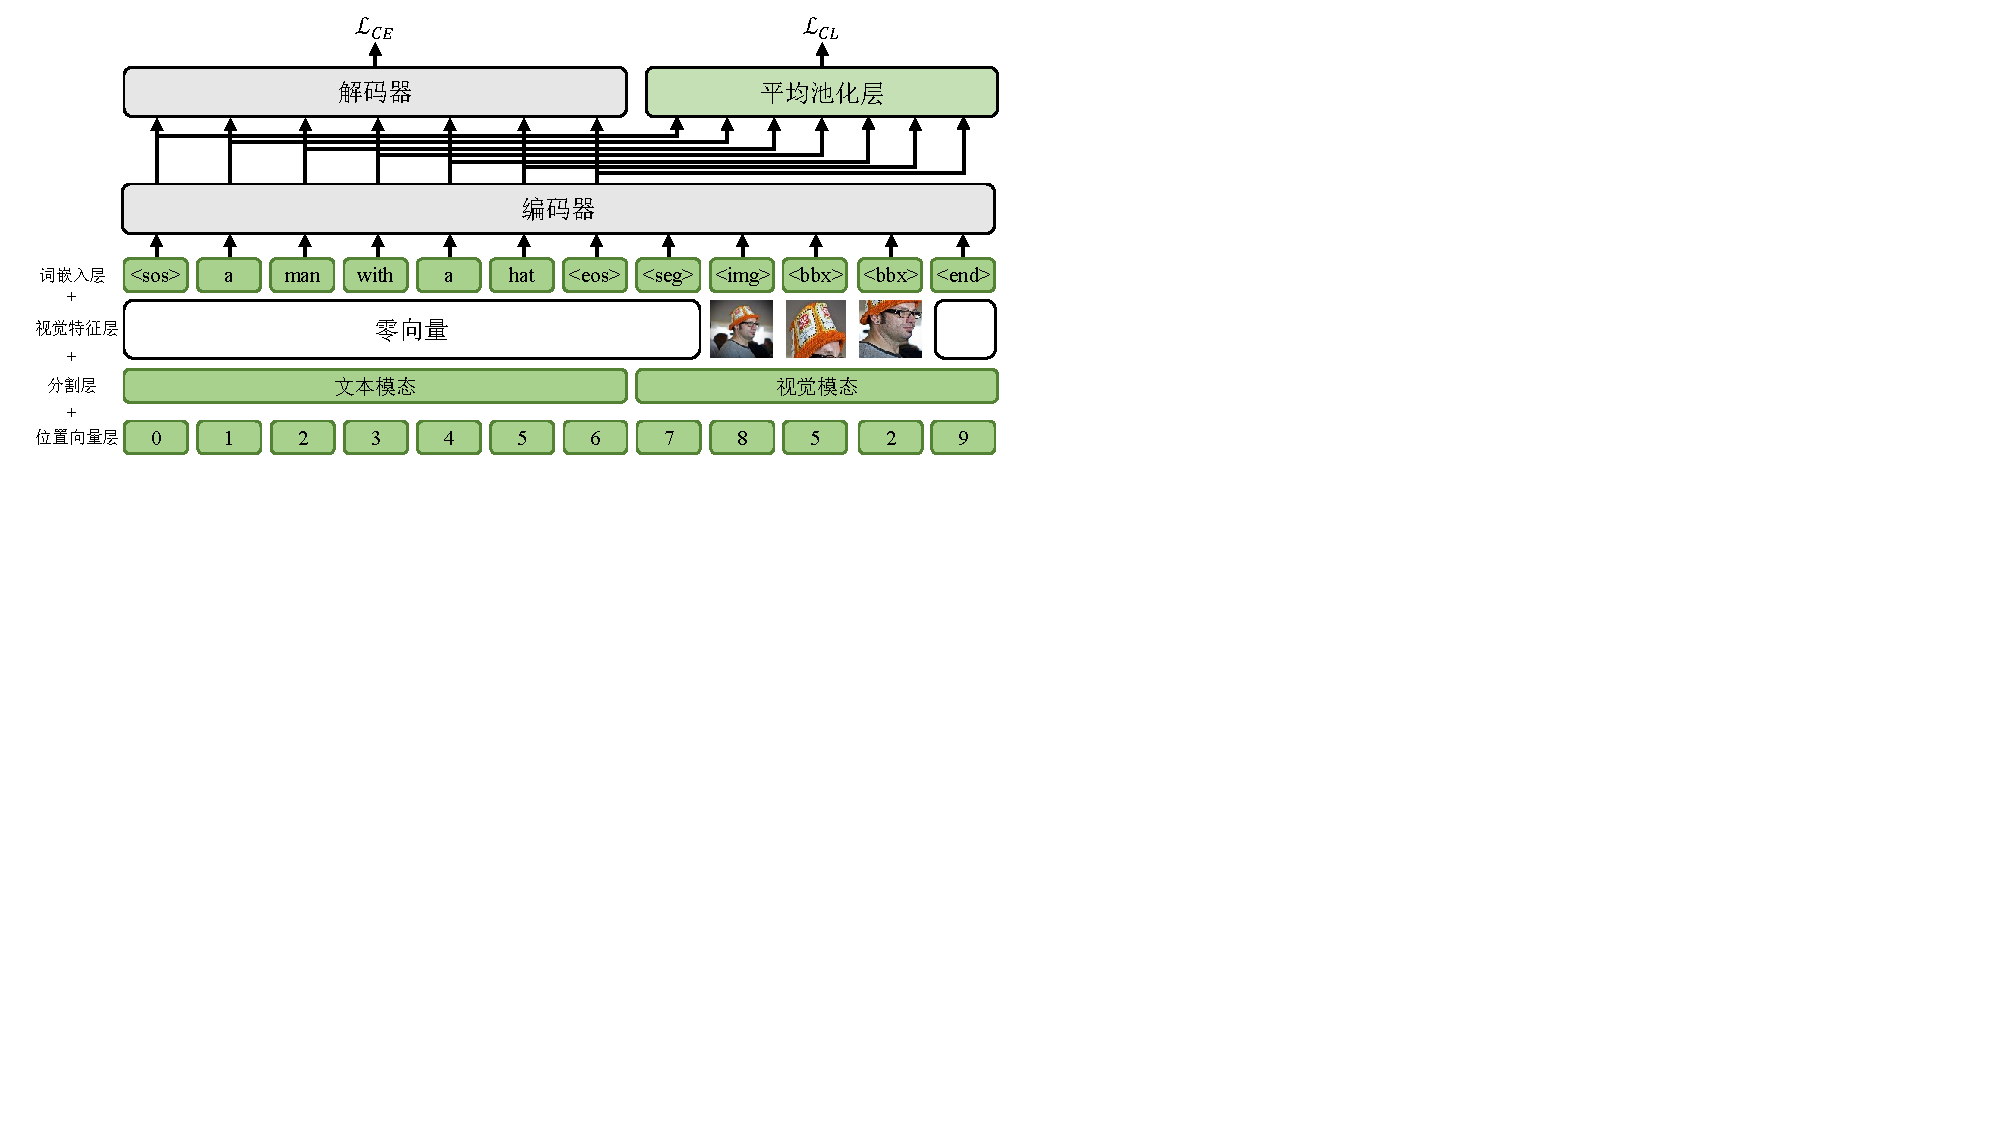
\includegraphics[scale=0.85]{Img/fig_5_model.pdf}
    \bicaption{结合对比对抗训练方法的神经机器翻译模型}{NMT model combined with contrastive adversarial training method}
    \label{fig:5_model}
\end{figure}
本章采用了一种句子级跨模态语义融合模型结构,其输入为一个文本序列,和一个可选的视觉输入,该视觉输入为文本序列对应的完整图片以及图片内部的数个视觉目标,如图\ref{fig:5_model}所示。该模型的编码器和解码器为常规的Transformer结构。其中,Transformer的编码器负责跨模态信息融合。为了使Transformer支持文本加图片形式的输入,本文采用了一个跨模态嵌入层。该嵌入层共分为4个子层:词嵌入层,视觉特征层,模态分割层,位置编码层。

(1){\sffamily 词嵌入层:}为了支持图片的输入,需要在词嵌入层对应的词表中,加入一些特殊字符:“<seg>”将词嵌入层输入的前后两部分分割为文本和视觉两个序列;“<img>”代表着放置完整图片的位置,每个输入序列仅一个;“<bbx>”代表放置图片中的视觉目标的位置,每个输入序列可以有多个;“<end>”代表着跨模态输入序列的结尾。


(2){\sffamily 视觉特征层:}该层每个位置的输入与词嵌入层的特殊字符相对应,其中“<img>”的对应位置放置输入的完整图片的全局特征,“<bbx>”对应位置放置视觉目标的全局特征,其它位置输入零向量。


(3){\sffamily 分割层:}这一层的作用相对简单,主要用作标识每个位置的输入属于文本序列还是图片序列。因此一共只有“文本模态”和“视觉模态”两个值,每个值都是与词嵌入层维度相同的向量。其中“<seg>”之前的文本序列均对应着“文本模态”,“<seg>”以及其后面的序列均为“视觉模态”。


(4){\sffamily 位置向量层:}这一层与一般的位置向量作用相似,能够表示输入序列中的绝对位置关系。区别在于,当输入的视觉目标与文本中的某些词有对应关系时,可以将视觉目标的位置设置为与其对应的词相同的位置,从而达到加强图片信息作用准确性的目的。如图\ref{fig:5_model}所示,图片输入序列中的“帽子”的绝对位置为5,与文本序列中的“hat”保持一致。

在解码阶段,解码器仅接收“文本模态”的编码结果作为输入。这是因为本章的CAT方法旨在帮助神经机器翻译模型将视觉信息融合到文本表示中。而该过程发生在编码阶段,即没有针对解码器采取翻译以外的优化方法。因此,基于常规的神经机器翻译模型对视觉信息不敏感的假设,其内部模块,如解码器,往往也会忽略视觉信息的输入。所以,将“视觉模态”部分的隐层单元传递给解码器是多余的。

图\ref{fig:5_model}中可以看到,CAT-NMT的目标函数包含了两个部分:融合图片信息的神经机器翻译所需的交叉熵(cross entropy,CE)损失函数和CAT所需的对比损失函数。其中交叉熵损失函数为:
\begin{equation}
    \mathcal{L}_{CE}(\phi, \theta, \psi)=-\sum_j^M \log p(y_j|y_{<j},X,I)
\label{eq:5_cross_entropy}
\end{equation}
其中,$y_j \in Y,j=1,\cdots,M$,$\phi$为解码器参数,$\theta$为编码器参数,$\psi$为跨模态嵌入层的参数。该损失函数与常规的图片信息辅助式神经机器翻译模型相似,均是通过源语言句子$X$和对应图片$I$为输入信息,生成翻译$Y$的形式。在本章的方案中,$I$代表了完整的图片信息,在模型输入中表示为完整图片和其中的多个视觉目标的组合。该损失函数无法反映出的信息是,本章的跨模态信息融合过程,仅发生在编码端。图\ref{fig:5_model}中除了平均池化(average pooling)层,其它参数均需要通过翻译任务来优化。

\subsection{对比对抗训练}
\label{sec:5_cat}
正如上一节介绍,本章是在Transformer的编码器中实现将图片信息或视觉目标信息融合到文本的表示中。然而,基于常规的神经机器翻译模型对视觉信息不敏感的假设,在没有额外的引导下,编码器同样会忽略图片信息的存在。为了有效地融合视觉信息,本章提出了图文对比对抗方法实现在编码过程将图片信息融合到文本的表示中。CAT方法主要包含三部分:对比学习,对抗训练以及双向翻译训练。

\begin{figure}[H]
    \centering
    \begin{subfigure}[b]{0.3\textwidth} % default 0.25\textwidth
    %\begin{minipage}[t]{0.33\linewidth}
      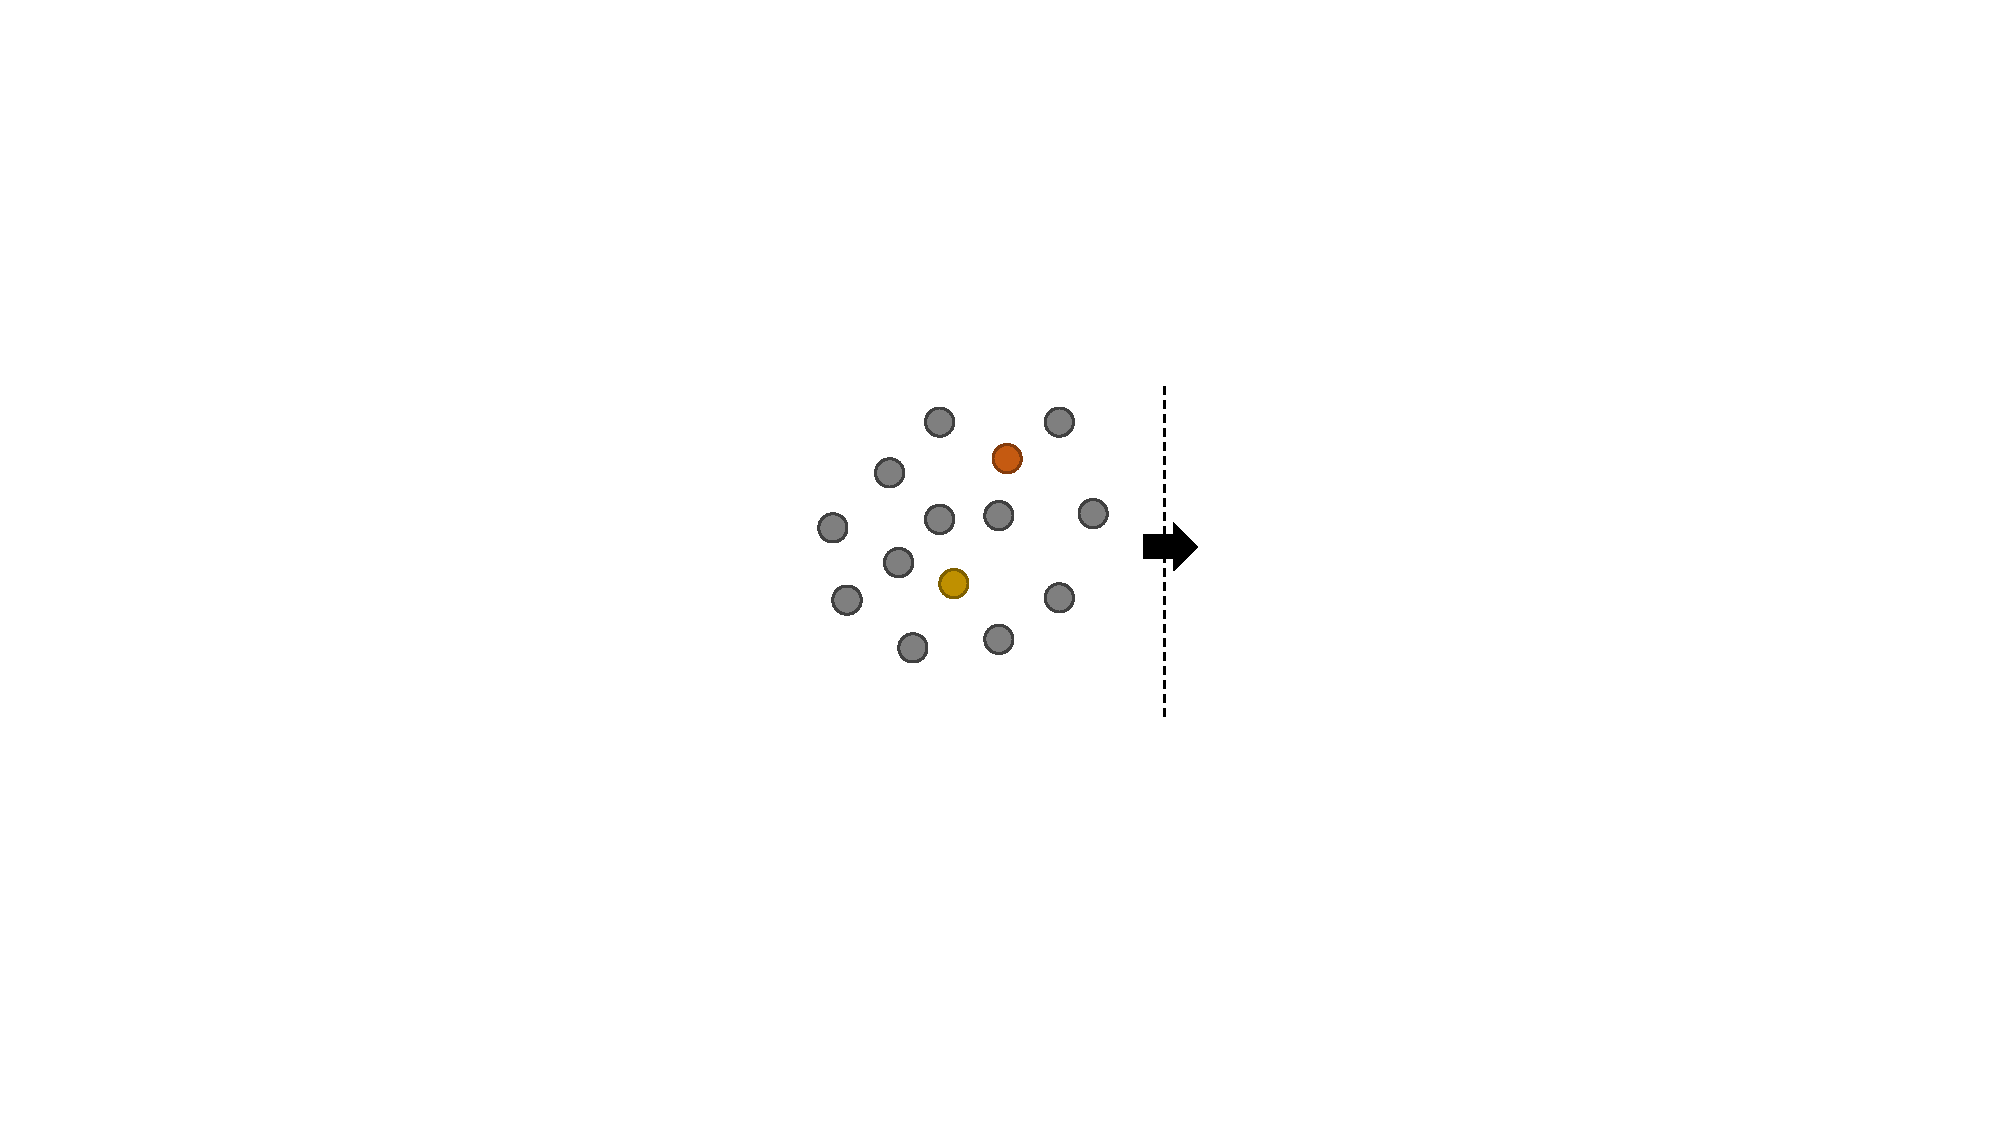
\includegraphics[width=\textwidth]{Img/fig_5_cat_a.pdf}
      \caption{}
      \label{fig:5_cat_a}
    %\end{minipage}
    \end{subfigure}%
    ~% add desired spacing
    \begin{subfigure}[b]{0.26\textwidth} % default 0.23\textwidth
    %\begin{minipage}[t]{0.33\linewidth}
      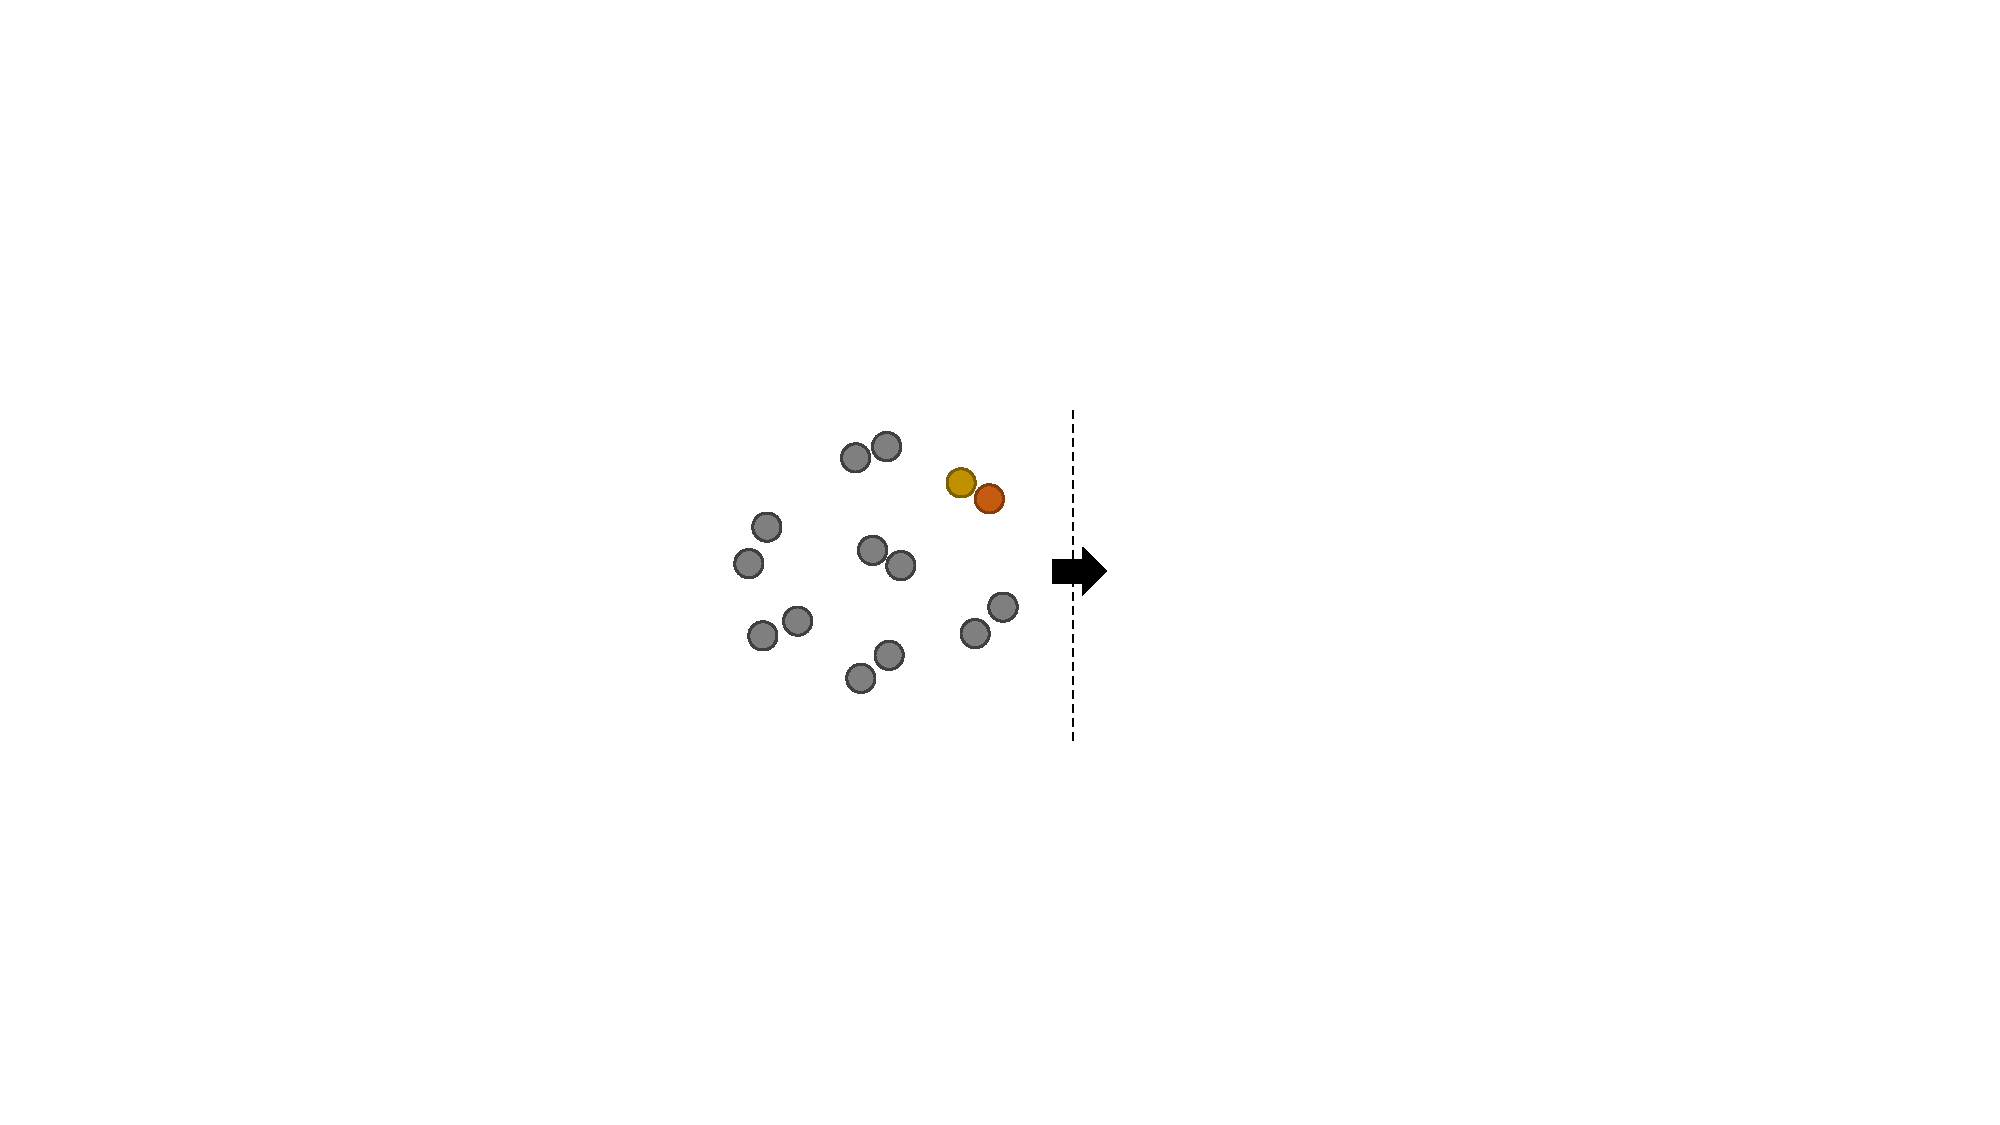
\includegraphics[width=\textwidth]{Img/fig_5_cat_b.pdf}
      \caption{}
      \label{fig:5_cat_b}
    %\end{minipage}
    \end{subfigure}
    % line break
    \begin{subfigure}[b]{0.38\textwidth} % default 0.32\textwidth
    %\begin{minipage}[t]{0.33\linewidth}
      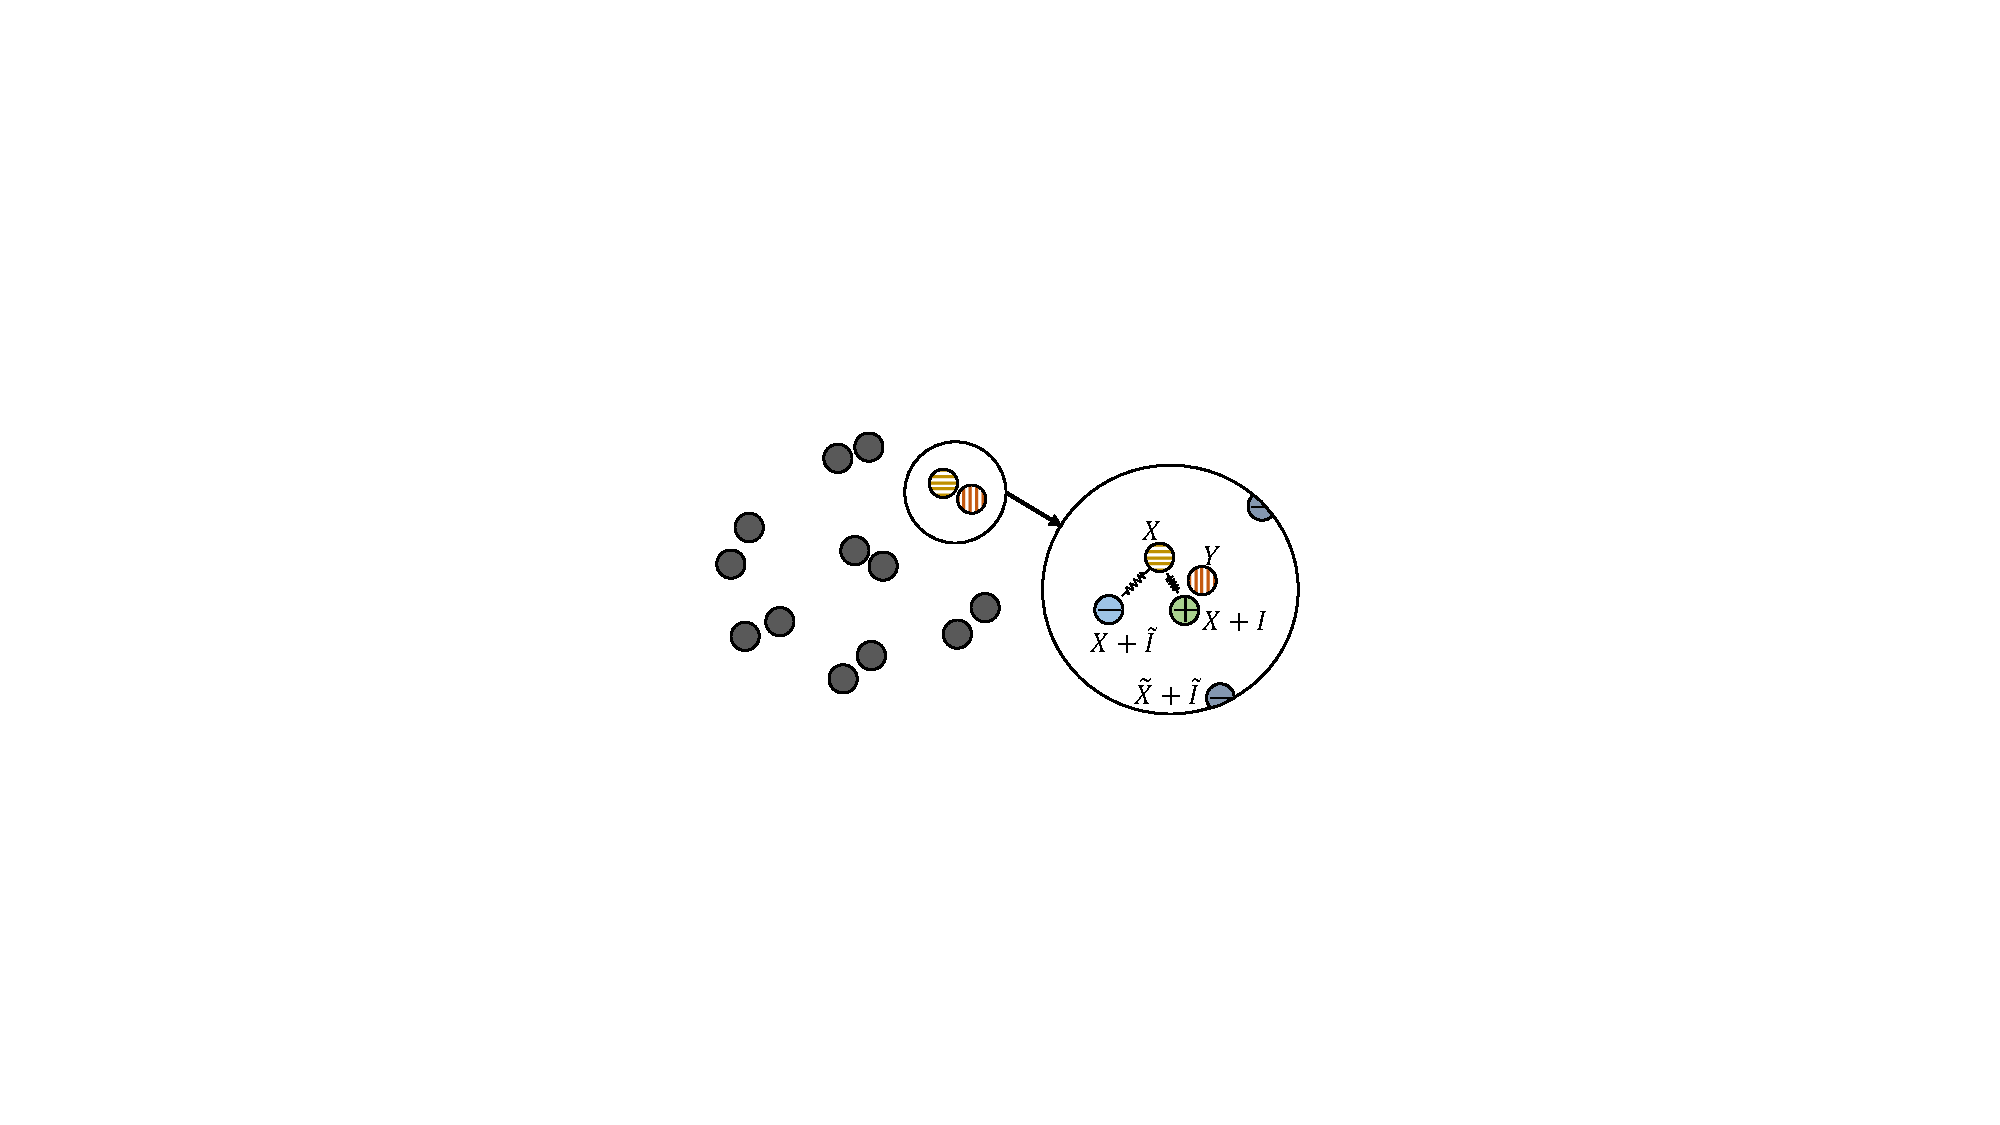
\includegraphics[width=\textwidth]{Img/fig_5_cat_c.pdf}
      \caption{}
      \label{fig:5_cat_c}
    %\end{minipage}
    \end{subfigure}%
    \bicaption{对比对抗训练方法原理示意图}{Schematic diagram of the principle of contrastive training method}
    \label{fig:5_cat}
\end{figure}

{\sffamily (1)对比学习}

对比学习方法能够在语义表示空间中拉近相似的样本,推离不相关的样本。在融合图片信息的神经机器翻译中,将目标译文$Y$作为锚点,将编码端的输入$X+I$作为正样本。在$X$与$Y$的双语统一表示空间中,对比学习方法能够拉近$X+I$与$Y$之间的距离,并将其它的所有样本视为负样本,拉开与$X+I$和$Y$之间的距离。图\ref{fig:5_cat}中每个圆代表文本语义表示空间的一个点,其中图\ref{fig:5_cat}(a)和图\ref{fig:5_cat}(b)展示了对比学习将表示空间的样本分簇归类的能力,图\ref{fig:5_cat}(b)中的每个簇可视为一个双语平行句对。常规的对比学习(contrastive learning,CL)损失函数为:
\begin{equation}
    \mathcal{L}_{CL}(\theta, \psi)=-\log\ \frac{e^{\mathrm{cos}(\mathrm{A}(Y),\mathrm{A}(X+V))/\tau}}{\sum_{Z\in N}e^{\mathrm{cos}(\mathrm{A}(Y),\mathrm{A}(Z))/\tau}}
    \label{eq:5_contrastive_learning}
\end{equation}

其中$\mathrm{cos}(\cdot,\cdot)$为余弦相似度函数,用于计算两个表示向量的语义相似度;$\tau$为温度,控制区分正负样本的能力;$\mathrm{A}(\cdot)$代表平均池化,正如图\ref{fig:5_model}所示,对比损失的输入是文本表示经平均池化后的结果;$N$代表着负样本集。

$\mathcal{L}_{CL}$与$\mathcal{L}_{CE}$之间共享编码器和跨模态嵌入层的参数,因此本章所采用的对比学习只针对编码器进行参数优化,从而使编码器具备利用图片信息辅助句子编码的功能。

{\sffamily (2)对抗训练}

尽管采用对比学习方法能够拉近相似样本$X+I$与$Y$之间的语义关系,并增加与其它样本之间的距离,但是该过程并不能保证翻译模型利用到了图片$I$中的信息。这是因为在机器翻译任务所使用的数据中,多数的原文$X$与译文$Y$都保持着良好的对齐关系。并且对于翻译任务所需要的信息而言,大部分$X$与$X+I$所能提供的语义信息的差距也很小。当模型对视觉信息不敏感时,即便输入的是$X+I$,模型仅通过输入中的文本信息$X$就可以得到相对可用的结果,且该过程相比于提取图片中的跨模态信息是更容易的。这一点对于融合跨模态信息的神经机器翻译和对比学习拉近语义关系均是通用的。

为了让模型具备融合视觉信息的能力,首先需要使模型具备更细粒度的语义聚类的能力。如图\ref{fig:5_cat}(c)所示,为了让模型区别出$X$与$X+I$之间的差别,就需要在原对比学习的基础上增加其它可对比的信息。因此,本章针对负样本集$N$进行了相应的改进:
\begin{equation}
    N=N_{AS}\cup B_{\setminus X}
    \label{eq:5_negative_sample_set}
\end{equation}
\begin{equation}
    N_{AS}=\{X+\tilde{I},\tilde{X}+\tilde{I}\}
    \label{eq:5_adversarial_sample_set}
\end{equation}
其中$\tilde{I}$为随机图片;$\tilde{X}$为退化句子,其内部与视觉目标相对应的词被替换为特殊字符“<mask>”;$B_{\setminus X}$代表同批数据中除$X$外的其它样本;$N_{AS}$为对抗样本集。

在对抗样本集$N_{AS}$中,$X+\tilde{I}$有着与$X$以及$X+I$更近的语义关系,$\tilde{X}+\tilde{I}$次之。但$N_{AS}$是负样本集的子集,此时带有源语言信息的$X$同时出现在正样本集和负样本集中。对比学习方法想要区分开正负样本就需要从输入文本以外的图片中获取差异化的信息。上一节中提到,解码器仅依靠“文本模态”的隐层表示生成译文。为了给解码器提供更好的编码结果,在对比学习阶段也仅采用“文本模态”的隐层表示作为输入。这意味着当模型的输入为$X+I$时,对比学习为了获取到图片带来的差异化信息,需要迫使编码器将图片$I$中的信息融合到文本$X$的隐层表示中。因此,为了使神经机器翻译利用到视觉信息,采用对比对抗训练方法时一方面需要将对抗样本加入到负样本集中,另一方面需要保证视觉信息融合到文本的隐层表示中。

{\sffamily (3)双向翻译训练}

在公式(\ref{eq:5_contrastive_learning})中可以观察到,计算对比损失时,译文$Y$作为锚点同样需要参与计算过程。这表示Transformer的编码器不仅负责源语言端的文本加图片的编码,还要支持目标端语言的纯文本编码。然而,在一个常规的单向翻译任务中,仅源端语言在编码器中得到了优化。在本章所提方法中,源语言的编码会通过翻译任务的目标函数$\mathcal{L}_{CE}$联合对比学习的目标函数$\mathcal{L}_{CL}$得到优化。而目标语言在编码器中仅能得到对比学习的目标函数的优化。这种不平衡的优化方式可能会对CAT方法带来负面效果。因此,需要采用双向翻译训练(bi-directional translation training,BDTT)解决这个问题。在训练的过程中,模型将用于两个翻译方向的训练。其中源语言到目标语言的训练是在编码端融合图片信息的翻译训练,目标语言到源语言的训练是纯文本的训练过程。需要注意的是,BDTT方法影响的是目标语言的编码质量。没有BDTT的情况下,CAT方法依旧可以工作,只不过$\mathcal{L}_{CL}$损失函数需要从模型的初始随机状态优化目标语言的编码。

\subsection{与神经机器翻译结合}
\label{sec:5_combine_with_nmt}

为了得到联合损失函数,本文联合公式(\ref{eq:5_cross_entropy})与公式(\ref{eq:5_contrastive_learning})得到:
\begin{equation}
    \mathcal{L}=\mathcal{L}_{CE} + \lambda|X|\mathcal{L}_{CL}
    \label{eq:5_combine_with_nmt}
\end{equation}
其中$\lambda$是平衡交叉熵损失和对比损失的超参数。$|X|$代表句子$X$的句长。因为$\mathcal{L}_{CL}$中需要对隐层单元经过平均池化层,所以$\mathcal{L}_{CL}$需要乘以句长$|X|$从而与$\mathcal{L}_{CE}$同为句子级别的计算结果。
\section{实验设置}
\label{sec:5_setup}

\subsection{实验数据}
\label{sec:5_datasets}

\begin{table}[!htbp]
    \bicaption{数据集情况统计结果}{Statistic results about datasets}
    \label{tab:5_datasets}
    \centering
    \footnotesize% fontsize
    \setlength{\tabcolsep}{4pt}% column separation
    \renewcommand{\arraystretch}{1.2}%row space 
    \begin{tabular}{cccccc}
    \hline
    数据集 & 翻译任务 & 训练集 & 验证集 & 测试集 & 平行句对数量 \\\hline
    Multi30K\pcite{elliott2016multi30k}          & EN$\rightarrow$DE   & 29,000 & 1,014 & 1,000/1,000/461 & 32,475  \\
    Flickr30KEnt-JP\pcite{nakayama2020flickr30kentjp}   & EN$\rightarrow$JP   & 29,783 & 1,000 & 1,000           & 158,915 \\
    HVG\pcite{parida2019hindi}               & EN$\rightarrow$HI   & 28,932 & 998 & 1,595/1,400     & 32,925  \\
%    CLT-MMT bi $\cup B_{\setminus X}$ & 38.5  & 57.5  & 31.0  & 51.9  & 27.5  & 47.4  \\
%    CAT-MMT bi $\cup B_{\setminus X}$ & 38.5  & 57.5  & 31.0  & 51.9  & 27.5  & 47.4  \\
     \hline
    \end{tabular}%
\end{table}%

为了验证方法的有效性,本章分别在三个语言对上进行了测试,包括英德翻译(EN-DE)、英日翻译(EN-JP)和英印翻译(EN-HI)。这些数据集的数据统计情况如表\ref{tab:5_datasets}所示,其详细介绍如下:

(1){\sffamily 英德翻译:}Multi30K是融合图片信息的神经机器翻译任务普遍采用的数据集。该数据集中每张图片对应一句英文描述和一个德文翻译,并划分为训练集、验证集和测试集三部分,其中测试集又分为Test2016、Test2017和ambiguous MSCOCO 2017三个测试集。ambiguous MSCOCO 2017是专门针对歧义词问题设计的测试集。\ref{sec:5_architecture}小节中提到,可以为视觉目标与文本中的对应词提供相同的位置向量。针对Multi30K数据集,本章采用Flickr30K Entities提供的视觉目标与文本短语的实体对齐关系,文本中的对应词仅选择对应短语中的名词。由于Flickr30K Entities没有为Test2017和ambiguous MSCOCO 2017两个测试集提供实体对齐关系,因此我们采用\ref{sec:3_entity_extraction}节应用的视觉目标提取工具获得该对齐关系。本章采用Moses SMT\cite{44_koehn-etal-2007-moses}工具包对数据进行分词(tokenization)和归一化(normalization)处理。为了防止对视觉目标与名词对应关系的破坏,本章并没有采用双节编码技术\cite{27_sennrich-etal-2016-neural}(byte pair encoding, BPE)或WordPiece\cite{28_DBLP:journals/corr/WuSCLNMKCGMKSJL16}进行分词操作。

(2){\sffamily 英日翻译:}Flickr30KEnt-JP与Multi30K都是源自Flickr30K数据集。因此两者所使用的图片是一样的,区别在于Flickr30KEnt-JP是将Flickr30K的5个英文描述都翻译到了日文。所以该数据集中每张图片对应了5个英文描述和5个对应的日文翻译。相应地,也对该数据集的训练集、验证集和测试集的数据划分做了改变。

(3){\sffamily 英印翻译:}英语到印地语的翻译任务采用了HVG(Hindi Visual Genome)数据集。该数据集的图片来源于Visual Genome数据集。区别于Multi30K和Flickr30KEnt-JP,HVG中的每段英文描述是针对图片中的一个区域,这意味着其英文描述相对更短更简单。另外,该数据集提供了每段描述在图片中对应的区域。HVG的测试集分为一个普通的测试集和一个挑战集,该挑战集中包含了大量歧义词,专门为歧义词问题设计。在实验过程中,我们将完整的图片输入到“<img>”的对应位置,将与描述相关的图片区域输入到“<bbx>”对应的位置。

\subsection{模型设置}
\label{sec:5_model_setup}

本章所提方法在基于Transformer的翻译模型基础上进行的实验。因模型参数规模受数据集的大小的限制,我们选择了小规模的参数设置。Transformer的词向量维度为128,隐层向量维度为256。编码器和解码器的层数均为4。多头注意力机制的头数为4。在训练过程中dropout设置为0.2。批数据大小设置为源语言以及目标语言最多不超过2000个单词。本章采用Adam优化器在模型的训练过程中进行参数优化其中$\beta_1=0.9$,$\beta_2=0.998$,$\epsilon=10^{-9}$。本章与文献\cite{5_DBLP:journals/corr/VaswaniSPUJGKP17}相同采用预热和衰减策略来提高学习率,预热步骤为4000,总训练步骤为80000,取训练完成后的模型参数用于测试。训练目标中设置平滑标签$\epsilon_{ls}=0.1$。以上模型参数与文献\cite{33_yin-etal-2020-novel}。

公式\ref{eq:5_contrastive_learning}中的$\tau$设置为0.1,公式\ref{eq:5_combine_with_nmt}中的超参数$\lambda$设置为0.3。在评估英德翻译的结果时,采用BLEU4\cite{42_papineni-etal-2002-bleu}和METEOR\cite{46_denkowski-lavie-2014-meteor}两个评估指标。英日翻译和英印翻译仅采用BLEU4作为评估指标。

\subsection{对比模型}

本章所选择的对比模型可分为两类:图片辅助式神经翻译模型和图片增强式神经翻译模型。图片辅助式神经翻译模型在生成翻译的过程中会以源语言句子和对应图片作为参考生成译文,图片主要起到辅助翻译过程的作用。图片增强式神经翻译模型则是利用图片中的视觉信息增强模型的表示能力,在测试阶段一般不需要图片输入。本章所选择的对比模型均是以Transformer作为基础模型结构:
\begin{itemize}
    \item \textbf{SerialAtt\cite{47_DBLP:conf/wmt/LibovickyHM18}:}该模型在解码过程中采用了多个交叉注意力串联的形式,每个交叉注意力模块对应了不同的信息来源。在融合图片信息的模型中,两个交叉注意力模块分别用于采集源语言和图片中的信息。
    \item \textbf{MMT-TF\cite{40_yao-wan-2020-multimodal}:}该工作设计了一种多模态注意力模块,该模块需要链接源语言句子的表示和图像特征作为自注意力模块的查询。
    \item \textbf{OVC\cite{48_DBLP:conf/aaai/WangX21}:}该方法设计的模型以视觉目标作为图片输入,并设计了以针对视觉目标的损失函数,通过对输入视觉目标进行掩码操作使模型对具有相关信息的图片视觉目标敏感,并忽略那些不相关的视觉目标。
    \item \textbf{GAMMT\cite{41_DBLP:journals/corr/abs-2103-08862}:}使用Gumbel-Sigmoid改造注意力机制,帮助翻译模型关注到图片中与文本内容更相关的区域。
    \item \textbf{GMMT\cite{33_yin-etal-2020-novel}:}该模型视源语言句子与图片中的视觉目标为一个多模态图结构,然后利用设计的基于图的跨模态编码器进行编码,最终解码出目标端句子。
    \item \textbf{CTR-NMT:}该模型为本文第3章所设计的方法,采用了词级实体替换方案利用独享解码器重构源语言,是一种图片增强式神经翻译模型。
    \item \textbf{CER-NMT:}该模型为本文第4章所设计的方法,采用了双向实体重构方法,是一种图片增强式神经翻译模型。
    \item \textbf{Transformer:}基于Transformer的单向纯文本神经翻译模型,其模型配置与\ref{sec:5_model_setup}节保持一致。
    \item \textbf{MM-Transformer:}该模型为本章所设计的不使用对比损失的神经机器翻译模型,该模型与一般的融合图片信息的翻译模型相似,为一个单向翻译模型。
    
\end{itemize}

\section{实验结果}

在实验结果的展示中,“CAT-NMT”代表本章提出的采用对比学习与对抗训练的模型,该模型没有使用\ref{sec:5_cat}小节介绍的BDTT方法。可增加双向翻译训练的模型有“Transformer”、“IGNMT”以及“CAT-NMT”三个模型,增加BDTT方法的模型记作“Transformer~+~BDTT”、“IGNMT~+~BDTT”和“CAT-NMT~+~BDTT”。

\subsection{翻译结果}
\label{sec:5_translation_results}
% Table generated by Excel2LaTeX from sheet 'trmmt'

\begin{table}[!htbp]
    \bicaption{在Multi30K英德翻译上的结果。}{Translation results on Multi30K EN-DE.}
    \label{tab:5_ende}
    \centering
    \footnotesize% fontsize
    \setlength{\tabcolsep}{4pt}% column separation
    \renewcommand{\arraystretch}{1.2}%row space 
    \begin{tabular}{llcccccc}
    \hline
    \multicolumn{2}{c}{\multirow{2}{*}{模型}} & \multicolumn{2}{c}{Test2016} & \multicolumn{2}{c}{Test2017} & \multicolumn{2}{c}{MSCOCO} \\\cline{3-8}
      &   & BLEU         & METEOR        & BLEU         & METEOR        & BLEU         & METEOR   \\\hline
    \multicolumn{2}{l}{~~~~SerialAtt \pcite{libovicky2018input}} & 38.7 & 57.2 & - & - & - & - \\
    \multicolumn{2}{l}{~~~~MMT-TF \pcite{yao2020multimodal}} & 39.5 & 56.9 & - & - & - & - \\
    \multicolumn{2}{l}{~~~~OVC \pcite{wang2021efficient}} & - & - & 32.4 & 52.3 & 28.6 & \textbf{48.0} \\
    \multicolumn{2}{l}{~~~~GAMMT \pcite{liu2021gumbel}} & 39.2  & 57.8  & 31.4  & 51.2  & 26.9  & 46.0  \\
    \multicolumn{2}{l}{~~~~GMMT \pcite{yin2020novel}}          & 39.8  & 57.6  & 32.2  & 51.9  & 28.7  & 47.6  \\
    \multicolumn{2}{l}{~~~~CTR-NMT}        & 39.7  & 57.5  & 32.9  & 51.7  & \textbf{29.1}  & 47.5  \\
    \multicolumn{2}{l}{~~~~CER-NMT}        & 40.2  & 57.8  & 32.5  & 52.0  & 28.3  & 47.1  \\\hline
    \multicolumn{8}{c}{本章所提方法} \\\hline
    \multicolumn{2}{l}{~~~~Transformer} & 38.5  & 57.5  & 31.0  & 51.9  & 27.5  & 47.4  \\
    \multicolumn{2}{l}{~~~~~~~~~~~~+BDTT} & 39.4  & 57.1  & 31.3  & 50.6  & 26.7  & 46.1  \\\hline
    \multicolumn{2}{l}{~~~~IGNMT} & 39.7  & 57.5  & 30.6  & 50.5  & 27.2  & 46.0  \\
    \multicolumn{2}{l}{~~~~~~~~~~~~+BDTT} & 40.0  & 57.7  & 31.6  & 51.0  & 27.7  & 46.8  \\\hline
    \multicolumn{2}{l}{~~~~CAT-NMT} & 39.8  & 57.6  & 30.6  & 50.3  & 26.6  & 45.6  \\
    \multicolumn{2}{l}{~~~~~~~~~~~~+BDTT} & \textbf{40.6}  & \textbf{58.7}  & \textbf{33.5}  & \textbf{52.6}  & 29.0  & 47.8  \\
%    CLT-MMT bi $\cup B_{\setminus X}$ & 38.5  & 57.5  & 31.0  & 51.9  & 27.5  & 47.4  \\
%    CAT-NMT bi $\cup B_{\setminus X}$ & 38.5  & 57.5  & 31.0  & 51.9  & 27.5  & 47.4  \\
     \hline
    \end{tabular}%
\end{table}%

表\ref{tab:5_ende}展示了本章提出的CAT方法在英德翻译上与其它方法的对比结果。

(1)IGNMT与纯文本的Transformer的实验对比中发现,增加了图片输入的IGNMT并没有带来全面的翻译准确率提升。在增加了BDTT方法后,两个模型的翻译准确率均有所提升。其中IGNMT~+~BDTT与Transformer~+~BDTT相比提升的更多,但两者之间的差距并不大。这部分的实验说明,简单地将图片输入给神经翻译模型很难为翻译带来有效的提升。

(2)在没有采用BDTT时,从CAT-NMT的实验结果可以看到,其翻译准确率相比于IGNMT并没有明显的差距。CAT方法为模型带来的增益甚至没有BDTT为IGNMT带来的多。CAT方法在单独使用时似乎是无效的。

(3)采用了BDTT的CAT-NMT在所有实验中的整体表现最佳。值得注意的是,仅采用CAT的CAT-NMT的整体表现是不如IGNMT;采用BDTT的IGNMT相比没有采用时有少许提升。如果在CAT-NMT~+~BDTT中CAT没有起到额外的增益作用,那么CAT-NMT~+~BDTT应该与IGNMT~+~BDTT的结果相近。但实际结果是,当既采用CAT又采用BDTT时,CAT-NMT~+~BDTT相比于IGNMT以及IGNMT~+~BDTT均有着显著的提升效果。该结果说明仅采用对比对抗训练难以在小规模的数据上实现细粒度的语义表示聚类。BDTT方法通过解决目标语言与源语言之间训练不平衡的问题,使CAT能够更容易起到作用。


\begin{table}[!htbp]
    \bicaption{英日翻译与英印翻译的实验结果}{Translation results of EN-JP and EN-HI}
    \label{tab:5_enjp_enhi}
    \centering
    \footnotesize% fontsize
    \setlength{\tabcolsep}{4pt}% column separation
    \renewcommand{\arraystretch}{1.2}%row space 
    \begin{tabular}{llccc}
    \hline
    \multicolumn{2}{c}{\multirow{2}{*}{模型}} & 英日翻译~~~~ & \multicolumn{2}{c}{英印翻译}\\\cmidrule(r){3-3} \cmidrule(r){4-5}%\cline{3-5}
           &        & 测试集  & 测试集  & 挑战集~~~~  \\\hline
    
    \multicolumn{2}{l}{~~~~Transformer}    & 38.7           & 47.8           & 44.2~~~~  \\
    \multicolumn{2}{l}{~~~~~~~~~~~~+BDTT} & 38.6           & 49.4           & 45.5~~~~   \\\hline
    \multicolumn{2}{l}{~~~~IGNMT}            & 38.6           & 50.2           & 45.7~~~~  \\
    \multicolumn{2}{l}{~~~~~~~~~~~~+BDTT}        & 38.4           & 50.6           & 45.7~~~~  \\\hline
    \multicolumn{2}{l}{~~~~CAT-NMT}       & 38.8           & 50.4           & 44.8~~~~  \\
    \multicolumn{2}{l}{~~~~~~~~~~~~+BDTT}     & \textbf{39.3}  & \textbf{52.0}  & \textbf{47.0}~~~~  \\
%    CLT-MMT bi $\cup B_{\setminus X}$ & 38.5  & 57.5  & 31.0  & 51.9  & 27.5  & 47.4  \\
%    CAT-NMT bi $\cup B_{\setminus X}$ & 38.5  & 57.5  & 31.0  & 51.9  & 27.5  & 47.4  \\
     \hline
    \end{tabular}%
\end{table}%
本章同样在英日翻译和英印翻译数据上进行了实验。表\ref{tab:5_enjp_enhi}展示了这部分的实验结果。区别于英德翻译,在英日翻译上采用BDTT的模型并没有得到更进一步的效果,在最终的模型结果上也仅得到了0.6个BLEU值的提升。在英印翻译上的实验效果与在英德翻译上的效果是相似的。从整体上看,对比对抗训练方法在与双向翻译训练方法的配合下,能够为模型带来稳定的翻译准确率的提升。

\subsection{消融实验}
\label{sec:5_ablation_study}
\begin{table}[!htbp]
    \bicaption{消融实验结果}{Experiment results of ablation study}
    \label{tab:5_ablation_study}
    \centering
    \footnotesize% fontsize
    \setlength{\tabcolsep}{4pt}% column separation
    \renewcommand{\arraystretch}{1.2}%row space 
    \begin{tabular}{cccccccccccccc}
    %\toprule[1pt]
    \hline
    \multicolumn{2}{c}{\multirow{2}*{模型}} & \multicolumn{6}{c}{英德翻译} &\multicolumn{2}{c}{英日翻译~~~~} & \multicolumn{4}{c}{英印翻译}\\\cmidrule(r){3-8} \cmidrule(r){9-10} \cmidrule(r){11-14}%\cline{3-8}
      &   & \multicolumn{2}{c}{Test2016}& \multicolumn{2}{c}{Test2017}& \multicolumn{2}{c}{MSCOCO}& \multicolumn{2}{c}{测试集} & \multicolumn{2}{c}{测试集} & \multicolumn{2}{c}{挑战集}  \\\hline
    
    \multicolumn{2}{l}{CAT-NMT~+~BDTT}   & \textbf{40.6}  &  & \textbf{33.5}  &  & \textbf{29.0}  &   & \textbf{39.3}  &  & \textbf{52.0}  &   & \textbf{47.0}  \\
    & \qquad -w/o $B_{\setminus X}$  & 40.0  & (-0.6)  & 31.0  & (-2.5)  & 27.4  & (-1.6)  & 38.7  & (-0.6)  & 50.7  & (-1.3)  & 44.5  & (-2.5)   \\
    & \qquad -w/o $N_{AS}$           & 39.9  & (-0.7)  & 32.0  & (-1.5)  & 27.8  & (-1.2)  & 39.0  & (-0.3)  & 51.2  & (-0.8)  & 45.6  & (-1.4)    \\\hline
    \multicolumn{2}{l}{CAT-NMT}      & 39.8  &         & 30.6  &        & 26.6  &         & 38.8  &         & 50.4  &         & 44.8  & \\
    & \qquad -w/o $B_{\setminus X}$  & 39.6  & (-0.2)  & 30.6  & (0.0)  & 27.0  & (+0.4)  & 38.4  & (-0.4)  & 50.5  & (+0.1)  & 44.5  & (-0.3) \\
    & \qquad -w/o $N_{AS}$           & 39.8  & (0.0)   & 30.9  & (+0.3) & 26.5  & (-0.1)  & 38.5  & (-0.3)  & 50.4  & (0.0)   & 44.6  & (-0.2)  \\
%    CLT-MMT bi $\cup B_{\setminus X}$ & 38.5  & 57.5  & 31.0  & 51.9  & 27.5  & 47.4  \\
%    CAT-NMT bi $\cup B_{\setminus X}$ & 38.5  & 57.5  & 31.0  & 51.9  & 27.5  & 47.4  \\

    
     \hline
    \end{tabular}%
\end{table}%
为了分析本章为对比对抗训练所设计的负样本在模型中是否起到了作用,本节将针对CAT-NMT和CAT-NMT~+~BDTT设置了消融实验。

实验结果如表\ref{tab:5_ablation_study}所示,其中“w/o $B_{\setminus X}$”代表同批数据下的其它样本从负样本集$N$中移除。该条件下,负样本集$N$的大小为$|N|=|N_{AS}|=2$。“w/o $N_{AS}$”代表将对抗样本从负样本集$N$中移除。没有了$N_{AS}$,CAT方法将退化为一般的对比学习方法,不再进行细粒度的语义聚类。

从表\ref{tab:5_ablation_study}中的结果可以看到,移除$B_{\setminus X}$或$N_{AS}$的实验设置对CAT-NMT~+~BDTT有着较大的影响,对CAT-NMT的影响则可以忽略不计。消融后的模型表现与表\ref{tab:5_ende}和表\ref{tab:5_enjp_enhi}中IGNMT和IGNMT~+~BDTT相似,即与常规的图片信息辅助式神经机器翻译模型相似。从该实验结果中可以得到以下两个结论:

(1)$B_{\setminus X}$是对比学习有效的一个先决条件,仅采用对抗样本集$N_{AS}$作负样本集,即使CAT方法与BDTT配合也无法达到理想的效果。在$B_{\setminus X}$的帮助下,模型可以在语义空间中进行粗粒度的语义聚类。从而将互为翻译的句子聚类到一起,将不同语义的句子分开。然而仅采用$B_{\setminus X}$的情况下模型的翻译准确率依旧不理想,这说明翻译模型还没有对视觉信息敏感。

(2)$N_{AS}$是对比对抗训练有效的原因。增加了对抗样本作为负样本后,模型需要进行更细粒度的语义聚类才能把对抗样本与正样本区分开。如果模型能够成功地区分$X+\tilde{I}$与$X+I$,那么就必须从图片中获得差异化的信息。而根据本章对解码模块以及对比学习模块的设计可知,对比学习模块能够感知到图片信息的唯一途径就是将其融合到文本的表示中。只有当图片中包含了与文本内容相近的语义信息时,才能将其作为正样本使其与译文的语义靠近。

综合以上实验结果与分析,当负样本集同时包含$B_{\setminus X}$或$N_{AS}$时,在双向翻译训练的配合下对比对抗训练方法能够为图片信息辅助式神经机器翻译模型带来有效的翻译准确率的提升。
%该实验结果说为负样本集增加对抗样本集$B_{\\X}$是有效的。在$B_{\\X}$的帮助下,对比损失能够在更细粒度的语义空间中进行语义的聚类,从而使模型将输入的图片信息融合到文本的表示中。

\subsection{双向翻译训练分析}
\label{sec:5_bdtt_analysis}

在前面小节的实验结果中,双向翻译训练方法为模型的翻译质量提升起到了关键的作用。因此,有必要针对BDTT实施进一步地分析,从而展示其真正的作用。为此,我们记录了CAT-NMT~+~BDTT和CAT-NMT在训练过程中输入样本之间的余弦距离的变化情况。该实验在Multi30K的验证集上每2000步的训练进行一次记录。在\ref{sec:5_cat}小节和\ref{sec:5_translation_results}小节中解释到,BDTT是通过优化编码器对目标语言句子$Y$的表示能力使CAT方法有效。因此,本小节将以$X+I$为基线,记录$X$、$Y$以及$X+\tilde{I}$这三者与$X+I$之间在训练过程中的余弦距离变化。

\begin{figure}[!htbp]
    \centering
    \begin{subfigure}[b]{0.5\textwidth}
      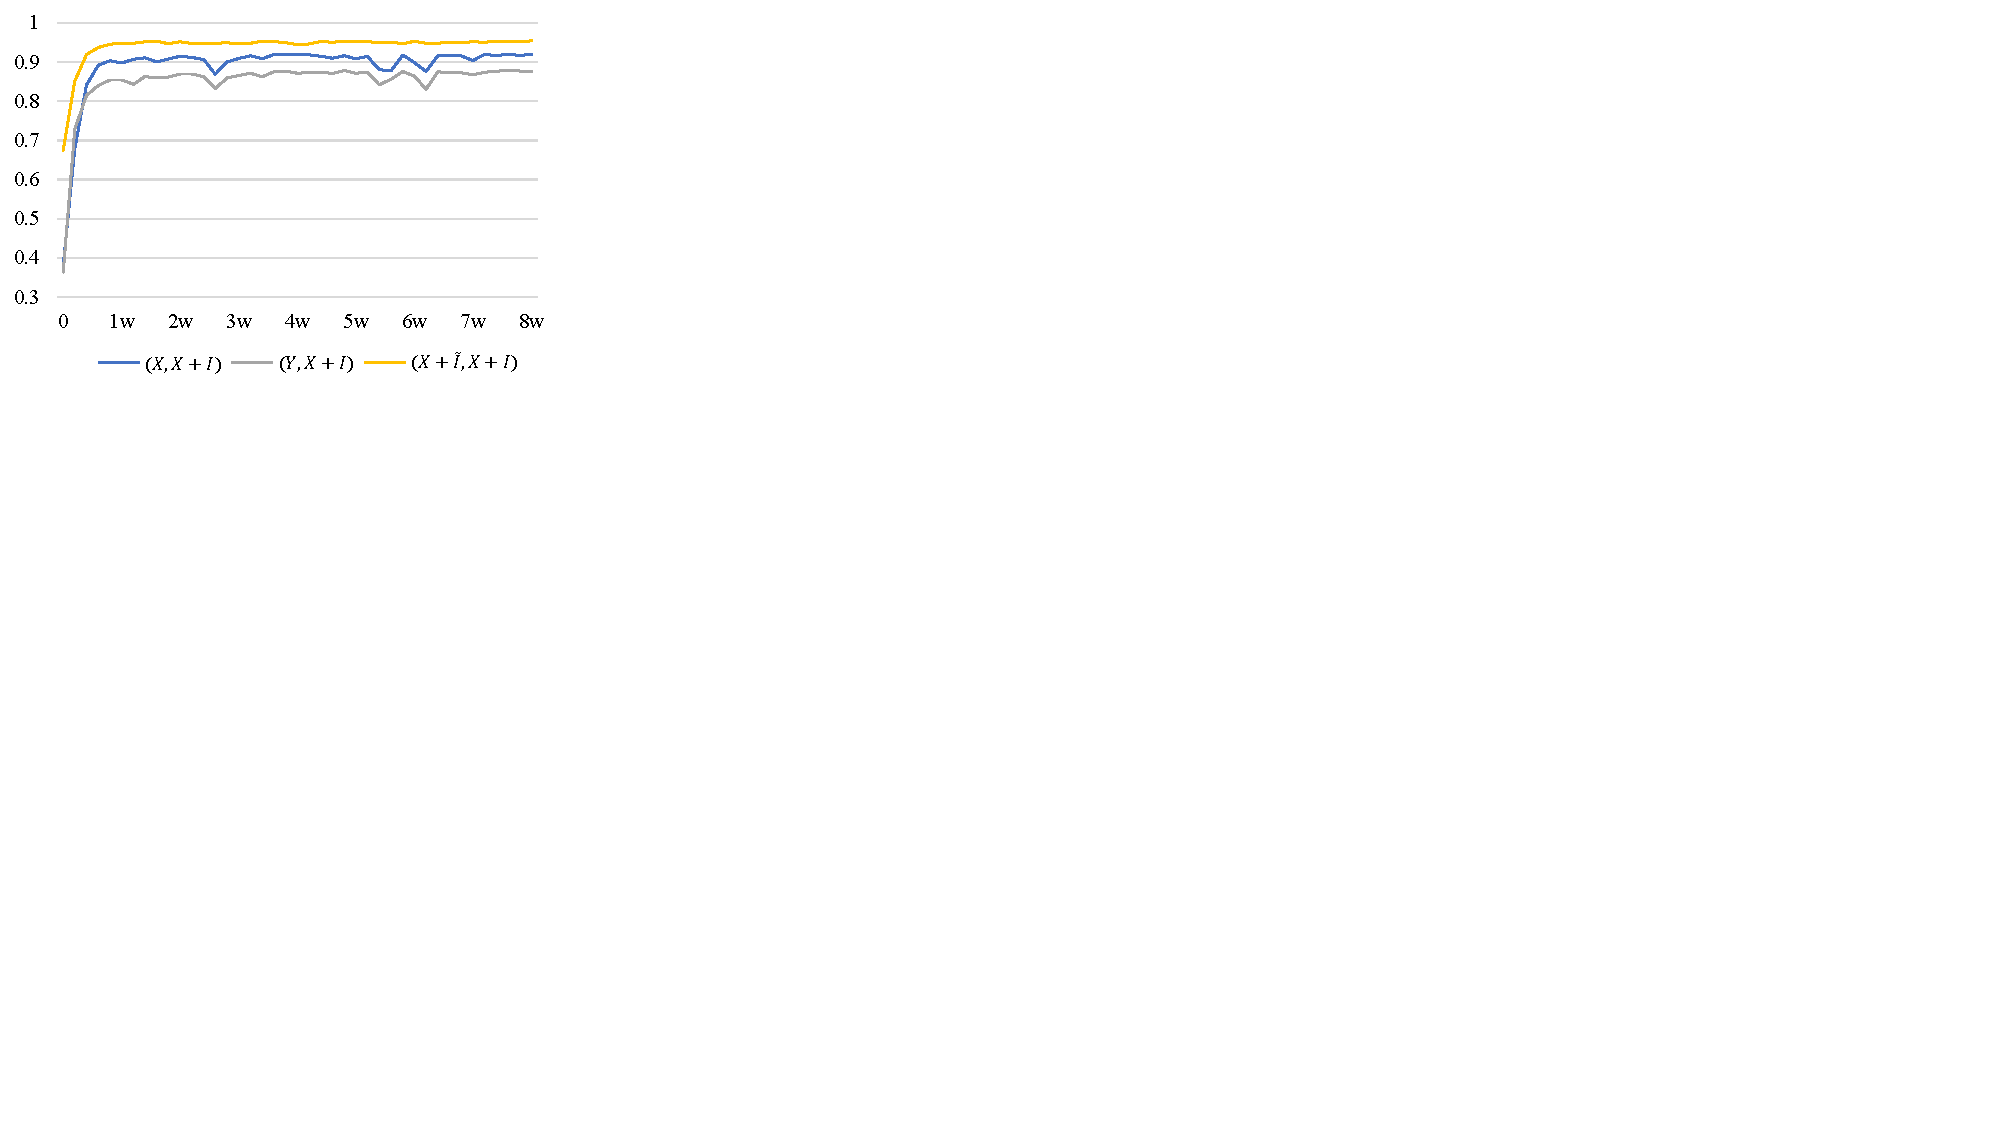
\includegraphics[width=\textwidth]{Img/fig_5_training_cat_mmt_bi.pdf}
      \caption{CAT-NMT~+~BDTT}
      \label{fig:5_training_cat_mmt_bi}
    \end{subfigure}%
    ~% add desired spacing
    \begin{subfigure}[b]{0.5\textwidth}
      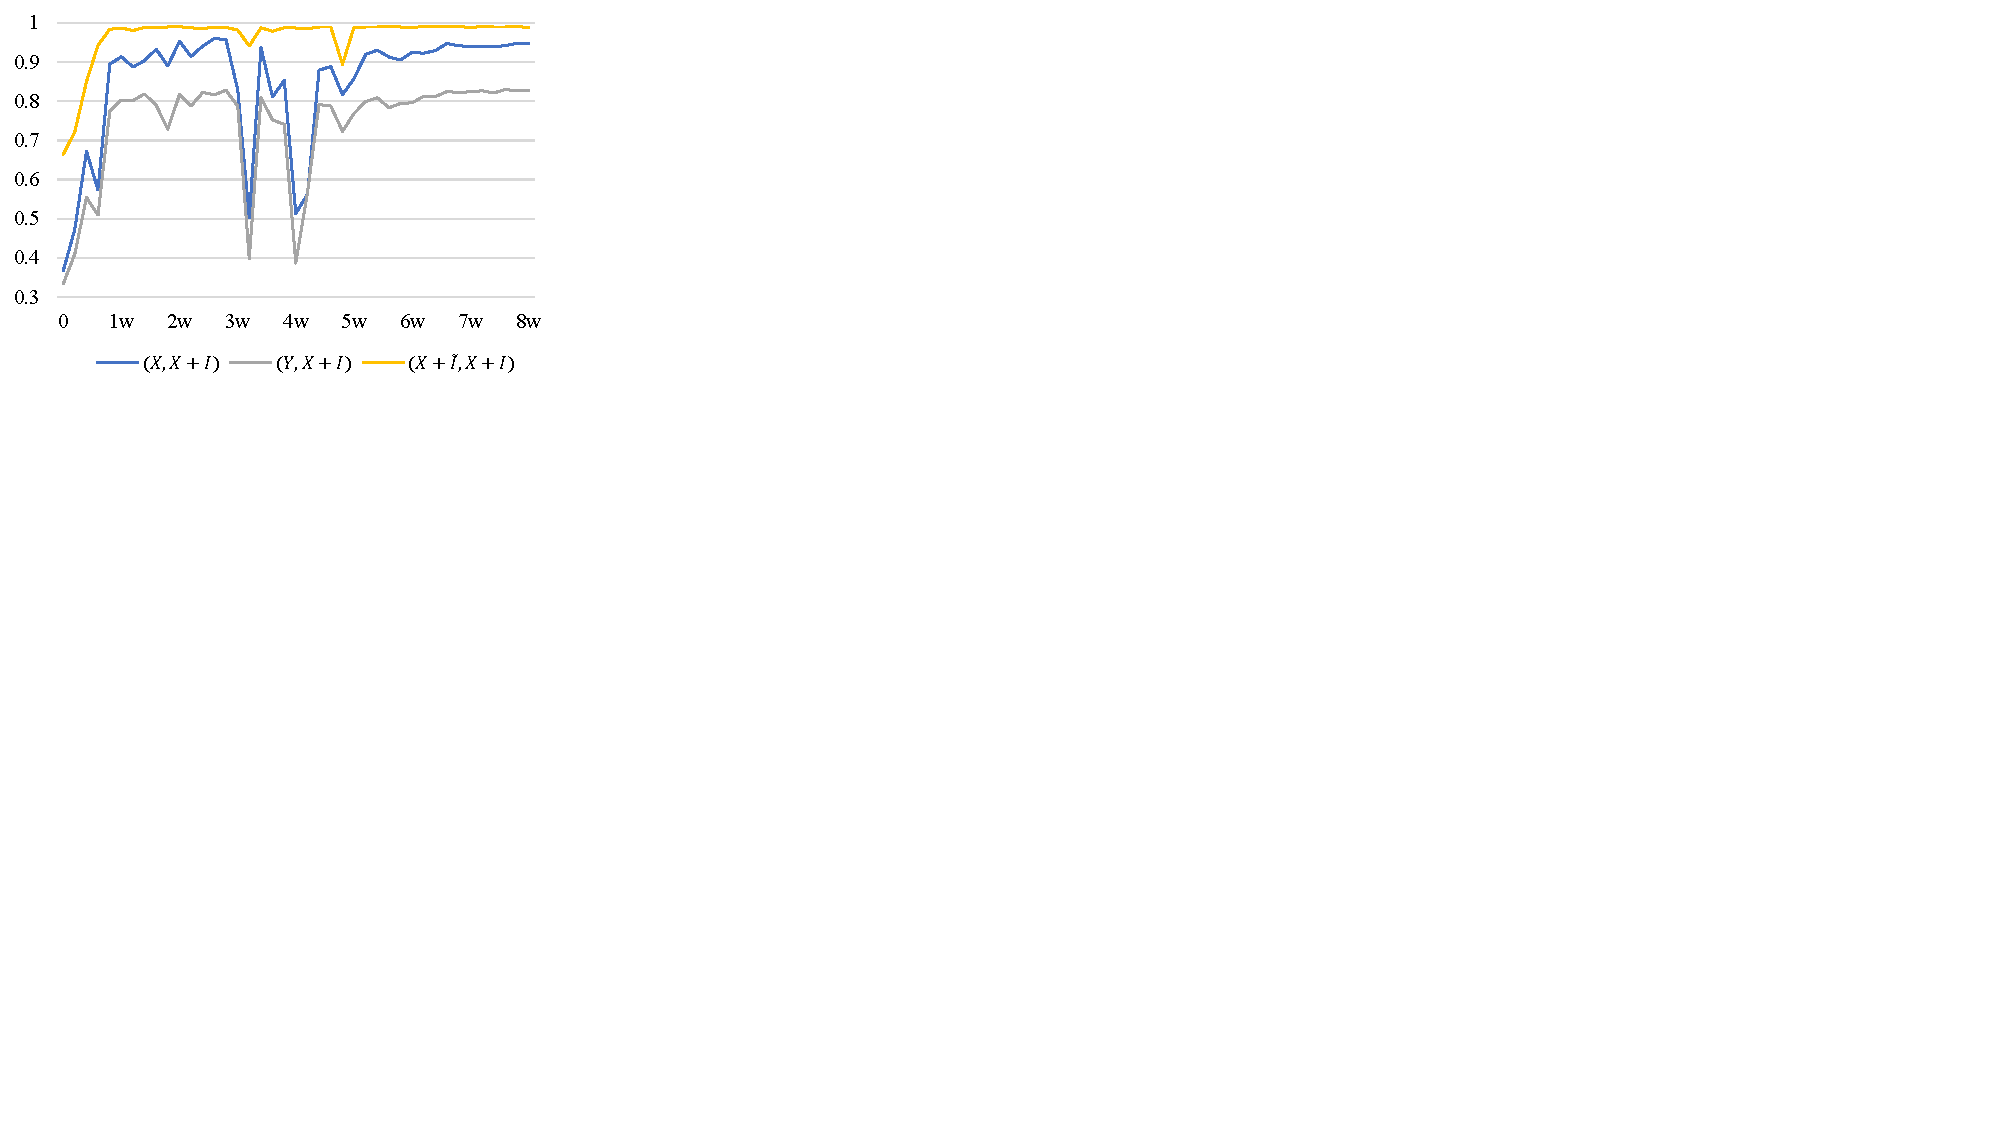
\includegraphics[width=\textwidth]{Img/fig_5_training_cat_mmt.pdf}
      \caption{CAT-NMT}
      \label{fig:5_training_cat_mmt}
    \end{subfigure}
    \bicaption{双向翻译训练方法在模型训练过程中对样本余弦距离的影响}{Influence of BDTT on cosine distance among samples during model training}
    \label{fig:5_training}
\end{figure}

实验结果如图\ref{fig:5_training}所示,其中$X+I$与$Y$之间的余弦距离在没有BDTT的情况下的收敛过程产生了急剧波动。这表明BDTT方法确实能够帮助目标语言得到好的编码表示。在仅使用CAT方法时,对比损失很难针对目标语言从开始训练一个好的表示向量。除以上观察外,该实验结果还可以得到以下结论:

(1)尽管在BDTT的配合下对比损失能够起到很好的作用,但$X+I$与$X+\tilde{I}$之间的余弦距离依旧很近(接近1.0)。这表明Multi30K验证集中的大部分句子并不需要视觉信息的帮助。这与我们的假设是一致的。

(2)图\ref{fig:5_training}(a)各样本之间的余弦相似度很快就收敛到了一个稳定的范围内。这说明在BDTT的帮助下,对比损失函数更像是对源语言和目标语言在表示空间的限制。使得在进行翻译优化的过程中,保持住样本之间的相对距离。

(3)$X$与$X+I$之间的余弦距离大于$X+\tilde{I}$与$X+I$之间。然而,$X$中并没有携带错误的图片信息,该结果实际上与预期相悖。一个可能的原因是,模型越多地关注“图片模态”中的信息,因为没有输入图片而导致的神经元连接的丢失所带来的负面影响就越大。这一点本文将在后面的小节中进一步证明。

(4)尽管相对距离最远的是目标语言$Y$,这样的结果也是可以理解的。在将目标端或源端句子的隐层单元传递给对比学习模块前,模型仅对隐层向量做了平均池化。在没有任何映射的情况下,将不同语言句子的平均表示向量映射到一个极度集中的区域内实际上是不太可能的。

\subsection{对抗评估}
\label{sec:5_adversarial_evaluation}
\begin{table}[htbp]
    \bicaption{对抗评估实验结果}{Experiment results of adversarial evaluation}
    \label{tab:5_adversarial_evaluation}
    \centering
    \footnotesize% fontsize
    \setlength{\tabcolsep}{3pt}% column separation
    \renewcommand{\arraystretch}{1.0}%row space 
    \begin{tabular}{lccccccccccccc}
    \hline
    \multicolumn{2}{c}{\multirow{2}*{模型}} & \multicolumn{6}{c}{英德翻译} & \multicolumn{2}{c}{英日翻译~~~~} & \multicolumn{4}{c}{英印翻译}\\\cmidrule(r){3-8} \cmidrule(r){9-10} \cmidrule(r){11-14}%\cline{3-8}
      &   & \multicolumn{2}{c}{Test2016}& \multicolumn{2}{c}{Test2017}& \multicolumn{2}{c}{MSCOCO}& \multicolumn{2}{c}{测试集} & \multicolumn{2}{c}{测试集} & \multicolumn{2}{c}{挑战集}  \\\hline
    
    CAT-NMT BDTT & $X+I$  & 40.6 &        & 33.5 &       & 29.0 &       & 39.3 &       & 52.0 &        & 47.0 & \\
    & $X$               & 40.3 &(-0.3)  & 32.1 &(-1.4) & 27.1 &(-1.9) & 38.7 &(-0.6) & 41.8 &(-10.2) & 35.5 &(-11.5) \\
    & $X+\tilde{I}$     & 40.4 &(-0.2)  & 31.6 &(-1.9) & 27.1 &(-1.9) & 38.9 &(-0.4) & 49.3 &(-2.7)  & 43.4 &(-3.6)  \\\hline
    IGNMT BDTT & $X+I$      & 40.0 &        & 31.6 &       & 27.7 &       & 38.4 &       & 50.6 &        & 45.7 & \\
    & $X$               & 39.6 &(-0.4)  & 30.8 &(-0.8) & 27.2 &(-0.5) & 38.2 &(-0.2) & 49.1 &(-1.5)  & 39.8 &(-5.9)  \\
    & $X+\tilde{I}$     & 39.9 &(-0.1)  & 31.6 &(0.0)  & 27.7 &(0.0)  & 38.5 &(+0.1) & 50.3 &(-0.3)  & 45.3 &(-0.4)  \\\hline
    
    CAT-NMT & $X+I$     & 39.8 &        & 30.6 &       & 26.6 &       & 38.8 &        & 50.4 &        & 44.8 & \\
    & $X$               & 38.9 &(-0.9)  & 30.3 &(-0.3) & 25.9 &(-0.7) & 38.7 &(-0.6)  & 48.6 &(-1.8)  & 35.8 &(-9.0) \\
    & $X+\tilde{I}$     & 39.4 &(-0.4)  & 30.5 &(-0.1) & 26.0 &(-0.6) & 38.9 &(-0.4)  & 50.0 &(-0.4)  & 44.1 &(-0.7)  \\\hline
    IGNMT & $X+I$         & 39.7 &        & 30.6 &       & 27.2 &       & 38.6 &        & 50.2 &        & 45.7 & \\
    & $X$               & 39.4 &(-0.3)  & 30.1 &(-0.5) & 26.7 &(-0.5) & 38.2 &(-0.2)  & 50.4 &(+0.2)  & 43.2 &(-2.5)  \\
    & $X+\tilde{I}$     & 39.6 &(-0.1)  & 30.5 &(-0.1) & 27.3 &(+0.1) & 38.5 &(+0.1)  & 50.1 &(-0.1)  & 45.7 &(-0.0)  \\
%    CLT-MMT bi $\cup B_{\setminus X}$ & 38.5  & 57.5  & 31.0  & 51.9  & 27.5  & 47.4  \\
%    CAT-NMT bi $\cup B_{\setminus X}$ & 38.5  & 57.5  & 31.0  & 51.9  & 27.5  & 47.4  \\

     \hline
    \end{tabular}%
\end{table}%
图片辅助式的神经机器翻译普遍存在着对视觉信息不敏感的问题,所以使用对抗样本评估模型对视觉信息的敏感度几乎成为每种方法必须经历的测试。本节将针对本章所提方法通过改变输入的图片测试模型对视觉信息的敏感度。其中“$X+I$”代表着为模型输入与原文对应的图片,“$X+\tilde{I}$”代表输入与原文不一致的图片,“$X$”代表只输入原文不输入图片。如表\ref{tab:5_adversarial_evaluation}所示为实验结果,从该实验结果中可以得到以下信息:

(1)对抗评估对CAT-NMT~+~BDTT带来的影响最大。这表明在BDTT的帮助下,CAT-NMT~+~BDTT能够从图片中获取信息从而带来翻译质量的提升。对抗评估对CAT-NMT的影响也有,但相对更小。从CAT-NMT在$X+\tilde{I}$和$X$两种输入下的结果中可以观察到,模型似乎只是对是否有视觉信息感兴趣,但对视觉信息中的内容并不感兴趣。

(2)相比于$X+\tilde{I}$,$X$对翻译准确率的负面影响更大。这一方面说明与原文不一致的图片作为一种噪声输入对模型是有一定正面的影响,例如提升模型的鲁棒性或做为一种正则方法提升了模型的翻译质量\pcite{wu2021good}。另一个原因是,当模型对输入图片中的视觉信息越敏感,模型在编码的过程中就越会“注意”“视觉模态”带来的信息。当输入为纯文本时,编码过程将丧失对“视觉模态”的神经元连接,在一定程度上造成了对纯文本输入不兼容的问题。因此带来的负面影响更严重。

(3)英德翻译的Ambiguous MSCOCO 2017和英印翻译的挑战集都是为歧义词问题而设计的。相比于其它的测试集,针对歧义词的测试集受对抗输入的影响更大。但对Ambiguous MSCOCO 2017的影响明显小于对英印翻译的挑战集,这说明尽管是针对歧义词而设计,但Ambiguous MSCOCO 2017内部的歧义词问题并不严重。该结果也解释了表\ref{tab:5_ende}中,CAT-NMT~+~BDTT在MSCOCO上的结果与CTR-NMT和CER-NMT之间差距不大的原因。

(4)英印翻译的HVG数据集受到对抗样本的影响最大。这是因为HVG数据集中对图片的描述更简单也更短,使得模型更容易做到跨模态的信息融合。然而,该结果同样表明了模型对视觉信息越敏感,模型的鲁棒性也就越差。面对对抗样本的攻击时,输出错误结果的概率就越大。

(5)尽管对抗样本降低了模型的翻译准确率,但是CAT-NMT~+~BDTT的结果依然超过了表\ref{tab:5_ende}和表\ref{tab:5_enjp_enhi}中纯文本模型的结果。这同样说明了噪音输入具有通过为模型提升鲁棒性提升翻译准确率的能力。这与\tcite{elliott2018adversarial,wu2021good}以及\tcite{li2021vision}的研究有着相似的结论。


\subsection{样例分析}
图\ref{fig:5_case_ende}、图\ref{fig:5_case_enjp}和图\ref{fig:5_case_enhi}分别展示了CAT-NMT~+~BDTT模型在三个不同的数据集上的翻译案例。本文选择了带有歧义词的句子,歧义词包含“passing”、“reached”以及“stamp”。为了方便比较,本节将模型的结果通过Google翻译系统\footnote{https://translate.google.com}翻译到了中文,并在每个句子下面展示。该实验结果表明了图片信息能够在很大程度上影响歧义词的翻译。在图\ref{fig:5_case_ende}英德翻译和图\ref{fig:5_case_enhi}英印翻译在$X+\tilde{I}$作为输入情况下出现了漏翻的问题。说明错误的图片信息影响到了歧义词的翻译过程。当纯文本$X$作为模型输入时,几乎所有的翻译结果都是错的,并与原来的词义相差甚远。这验证了我们之前的想法,说明模型越依赖视觉信息,其鲁棒性反而越差。

\begin{figure}[!htbp]
    \centering
    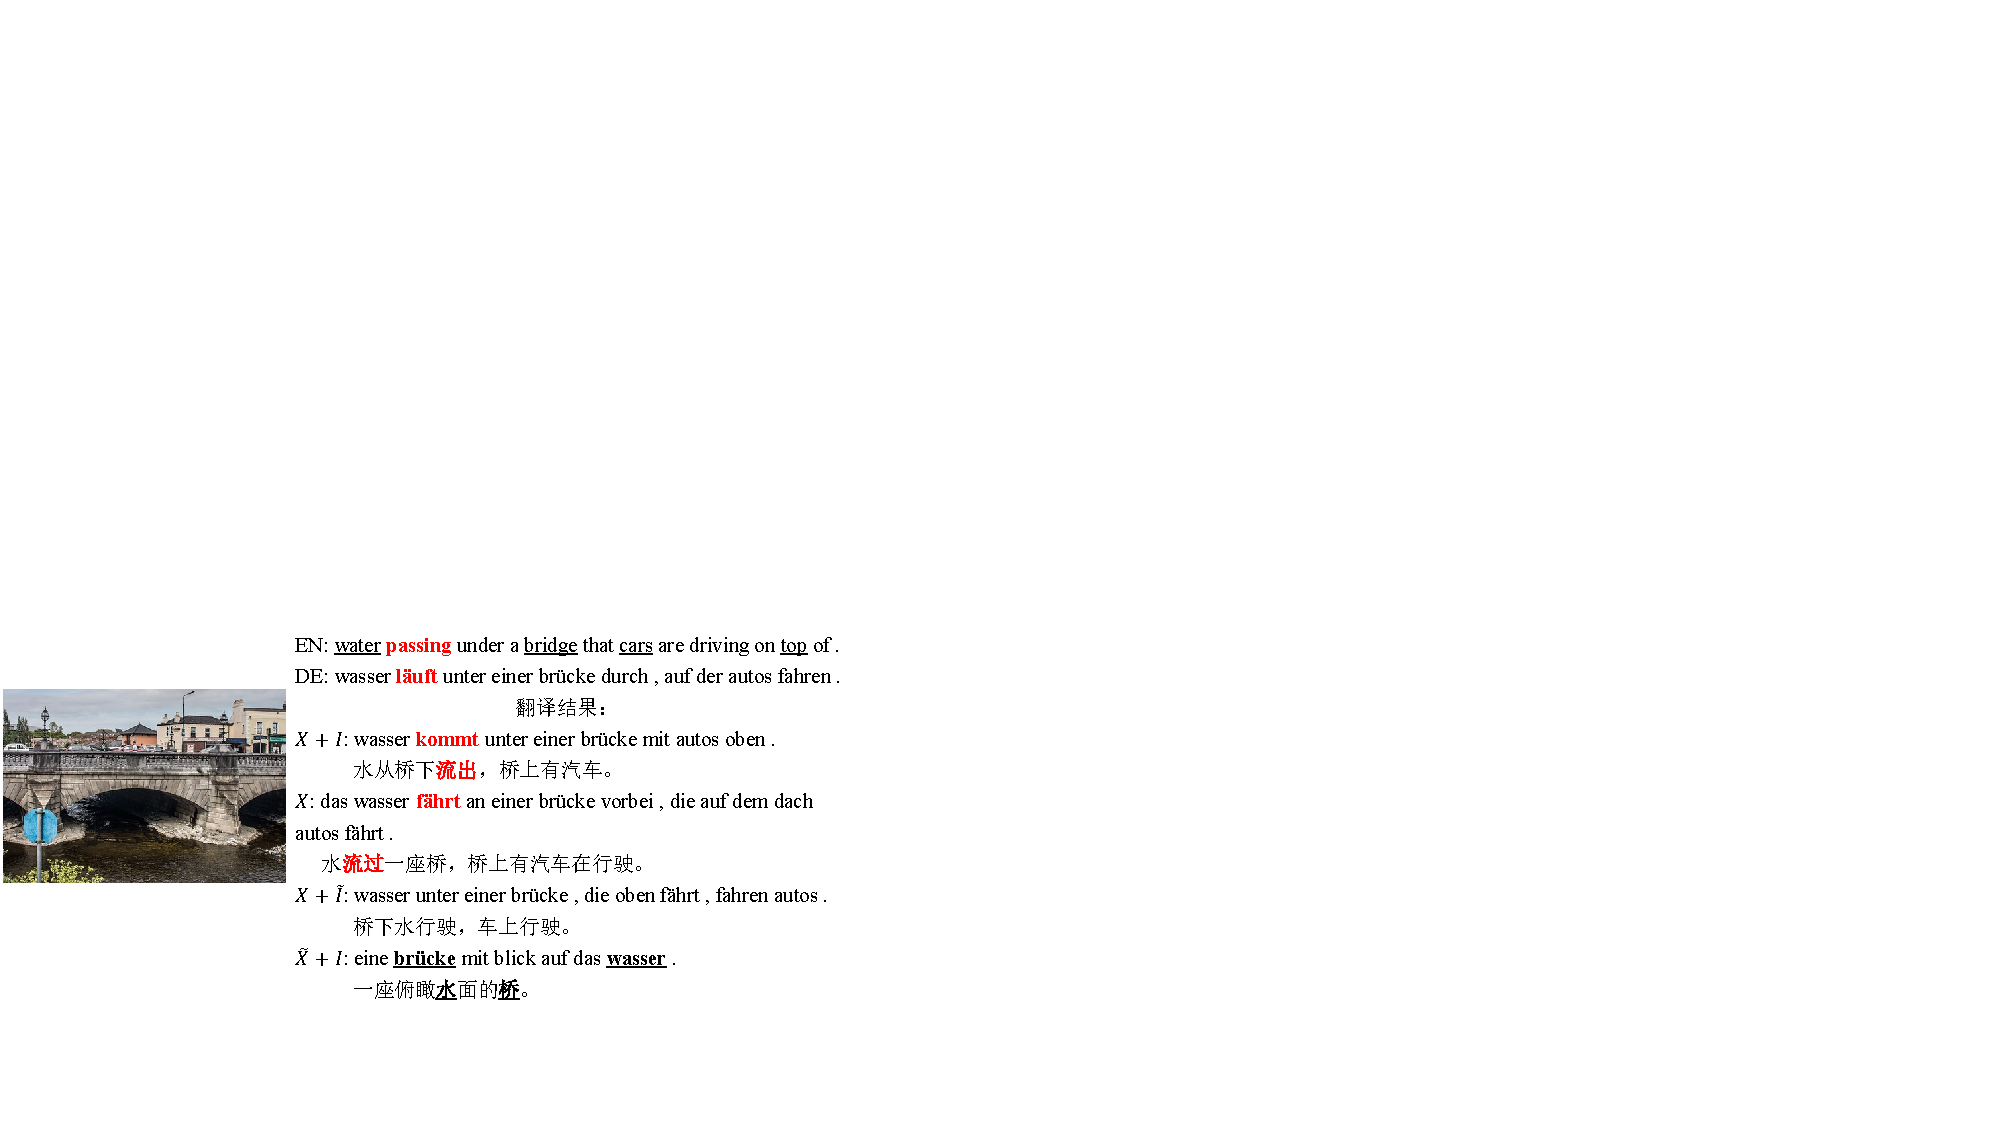
\includegraphics[scale=1.0]{Img/fig_5_case_ende.pdf}
    \bicaption{英德翻译案例}{Translation case for EN-DE}
    \label{fig:5_case_ende}
\end{figure}
\begin{figure}[!htbp]
    \centering
    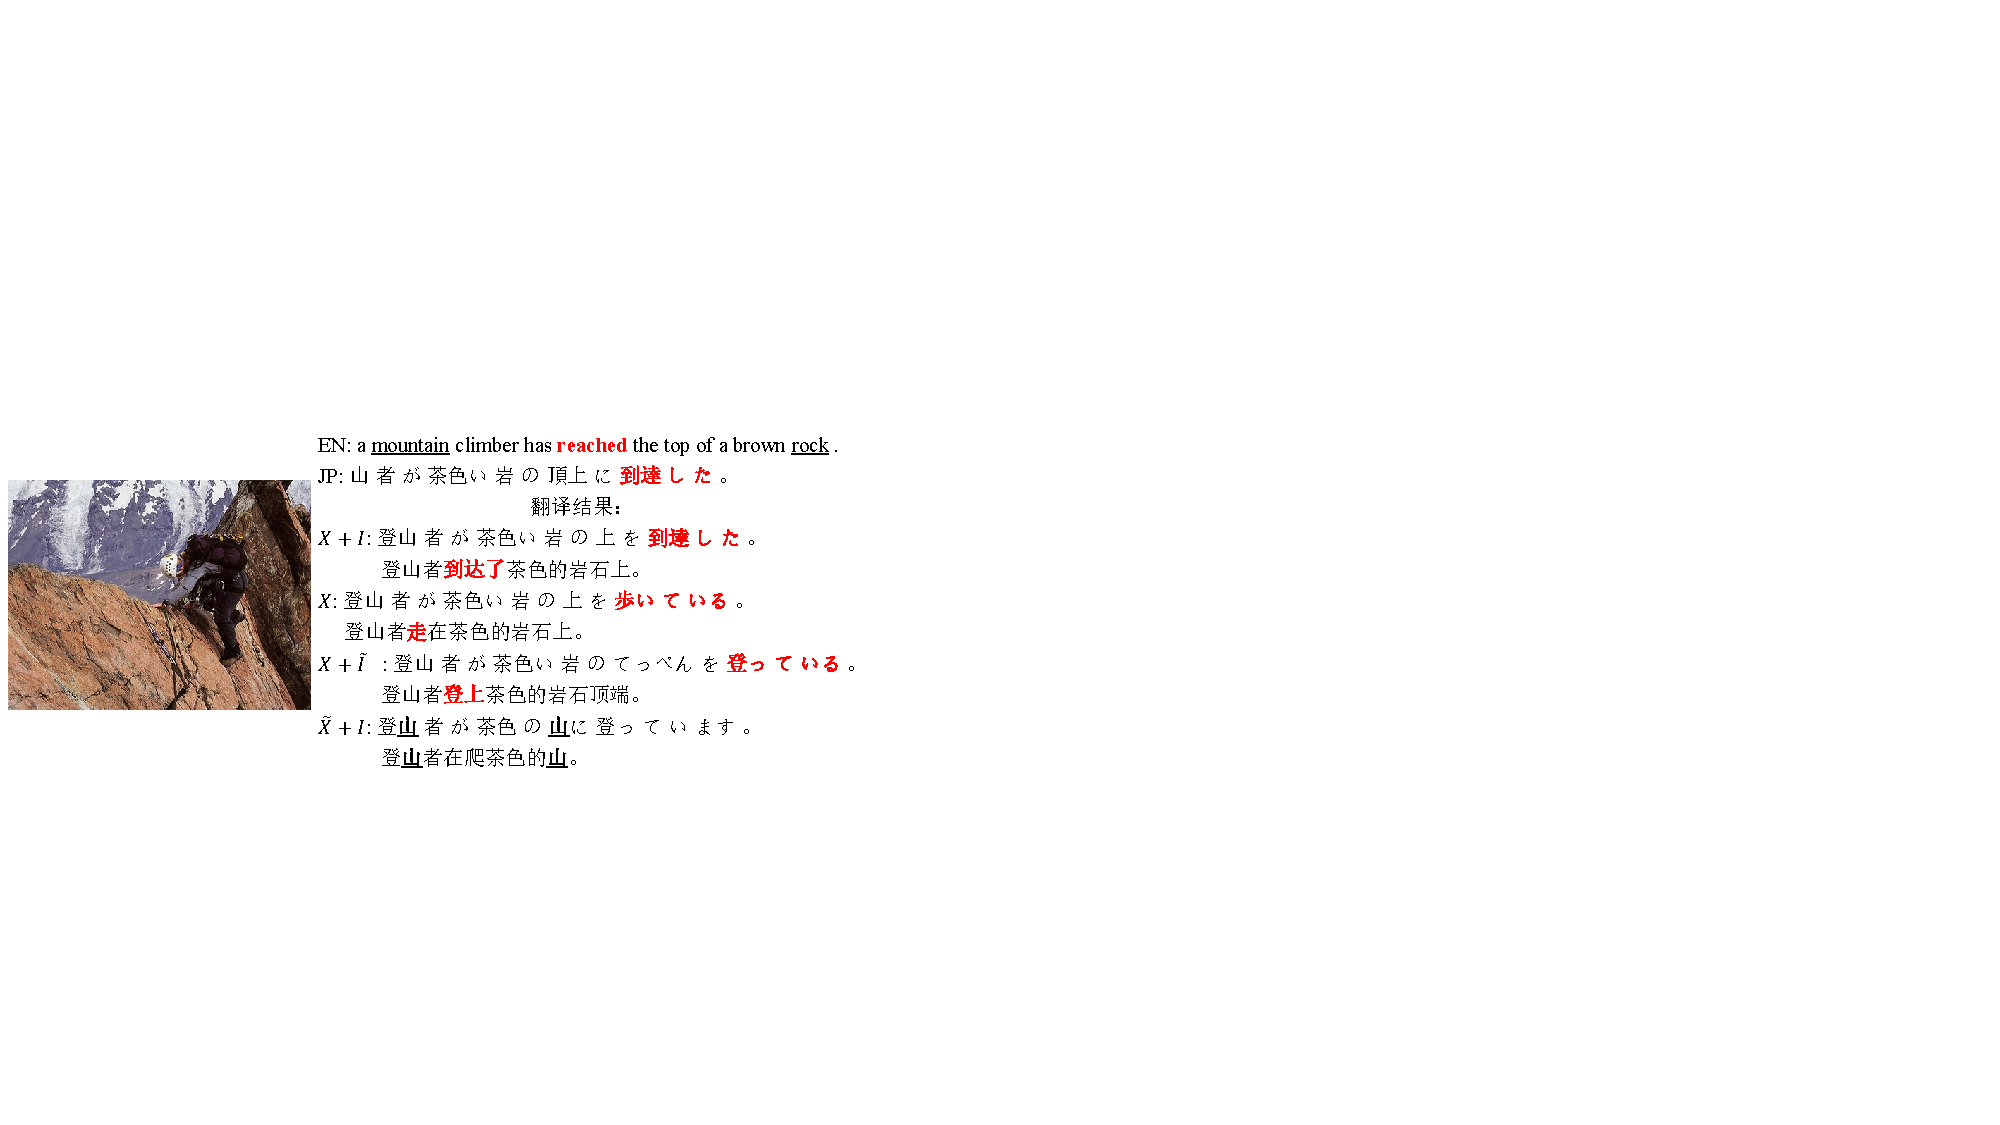
\includegraphics[scale=1.0]{Img/fig_5_case_enjp.pdf}
    \bicaption{英日翻译案例}{Translation case for EN-JP}
    \label{fig:5_case_enjp}
\end{figure}
\begin{figure}[!htbp]
    \centering
    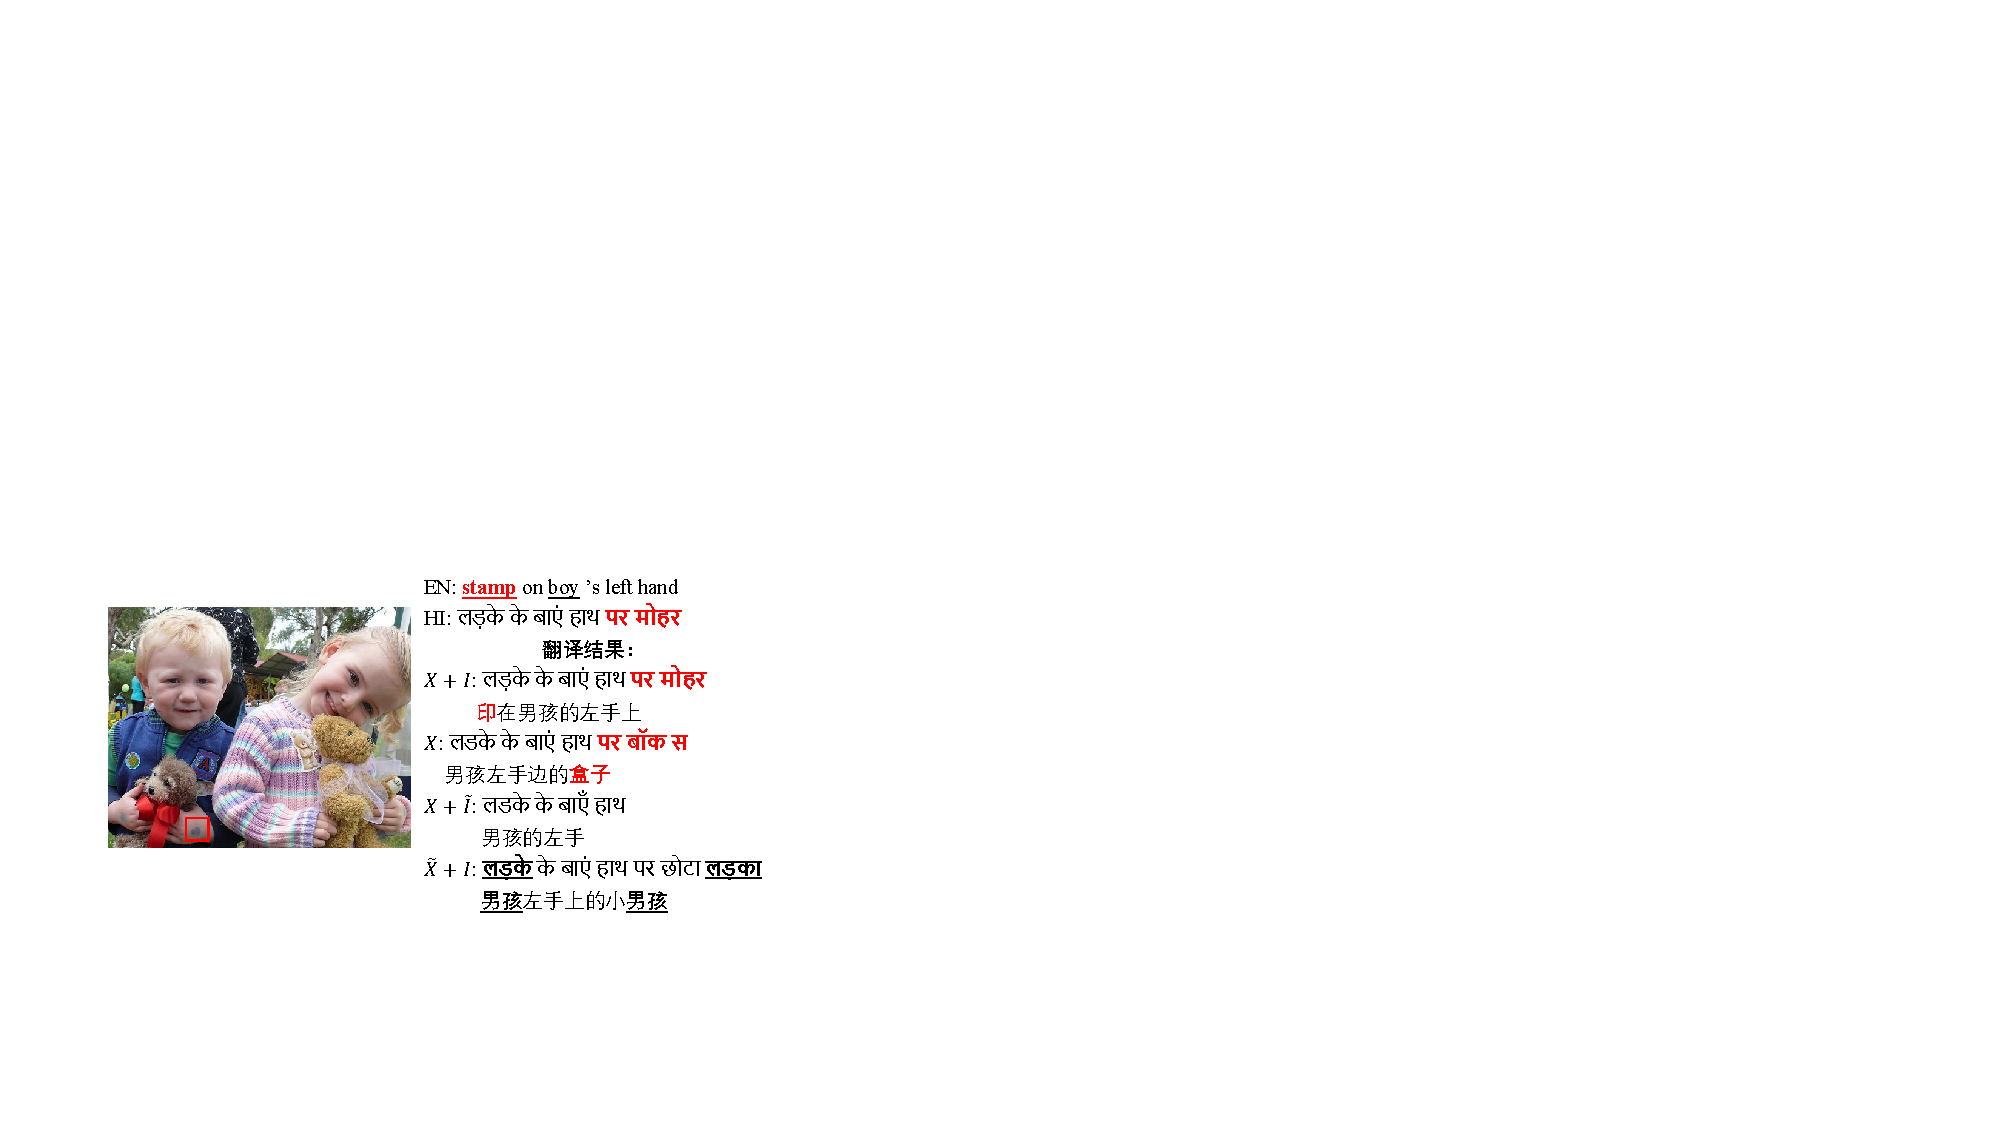
\includegraphics[scale=1.0]{Img/fig_5_case_enhi.pdf}
    \bicaption{英印翻译案例}{Translation case for EN-HI}
    \label{fig:5_case_enhi}
\end{figure}
我们还测试了模型在输入退化文本情况下通过图片补全信息的能力。文本的退化方案与\ref{sec:5_cat}小节中介绍的针对对抗样本$\tilde{X}+\tilde{I}$的方法相同,即将句子中与视觉目标相对应的名词替换为“<mask>”。图\ref{fig:5_case_ende}、图\ref{fig:5_case_enjp}和图\ref{fig:5_case_enhi}中所有源语言中带有下划线的词为选作退化的词。在$\tilde{X}+I$的翻译结果中重构出的对应词也同样带有下划线。图\ref{fig:5_case_ende}的结果显示,在图中有明显目标的“water”和“bridge”成功地在翻译中被还原。然而,整体的翻译结果却非常差。这是因为这个句子中有太多的词被掩码替换,破坏了整个句子的语义完整性,仅依靠图片很难补全完整的语义信息。图\ref{fig:5_case_enjp}中,为了降低难度,只选择了两个词“mountain”和“rock”。结果中“mountain”成功地还原了出来。但是根据源语言的句子,其还原出来的位置是错的。图\ref{fig:5_case_enhi}展示了一个简单的句子,“boy”成功地得到了还原,“stamp”则没有。

上述结果证明了本章所提方法将视觉信息融合到文本表示中的能力。当文本中出现歧义词时,模型可以准确翻译这些歧义词。替换或删除输入图像会极大地影响翻译结果。
上述分析还展示了机器翻译模型从匹配图像中还原退化句子缺失的信息的能力。模型可以从图像中捕获部分信息。实验结果还表明编码过程是文本主导的过程,输入文本的完整性在很大程度上影响翻译结果,图片信息只能起到辅助的作用。

\section{本章小结}
为了解决图片辅助式神经机器翻译对视觉信息不敏感的问题,本章提出了一种在对比学习中加入对抗样本的方法。在双向翻译训练方法的配合下,翻译模型以粗粒度的方式将不同的翻译句对聚类,以细粒度的方式区分翻译句对和对抗样本,从而实现了将输入图片中的信息融合到文本表示中。
本章在英德翻译、英日翻译、英印翻译和英中翻译四\sout{三}个数据集上进行了实验。实验结果表明,采用对比对抗训练的神经翻译模型能够有效提升神经机器翻译的翻译准确率。在消融实验中发现,在使用对比对抗训练方法时,对比学习所采用的负样本集是方法起作用的第一个条件,在负样本集中引入的对抗样本则是CAT方法有效的原因,在双向翻译训练方法的配合下,CAT方法能够提升翻译模型的性能。在进一步的对抗评估中发现,翻译模型在输入错误或不输入图片的情况下,模型的翻译性能有较大的波动,说明CAT方法使翻译模型对视觉信息更敏感。

该研究成果已被ACM亚洲语言与低资源语言信息处理周刊(TALLIP)接受。